\documentclass[12pt,a4paper]{report}
\usepackage[utf8]{inputenc}
\usepackage[T1]{fontenc}
\usepackage[french]{babel}
\usepackage{graphicx}
\usepackage{hyperref}
\usepackage{geometry}
\geometry{a4paper, left=2.5cm, right=2.5cm, top=2.5cm, bottom=2.5cm}
\usepackage{fancyhdr}
\usepackage{titlesec}
\usepackage{tabularx}
\usepackage{booktabs}
\usepackage{float}
\usepackage{caption}
\usepackage{listings}
\usepackage{xcolor}
\usepackage{enumitem}
\usepackage{array}
\usepackage{longtable}

% Configuration des couleurs pour le code
\definecolor{codegreen}{rgb}{0,0.6,0}
\definecolor{codegray}{rgb}{0.5,0.5,0.5}
\definecolor{codepurple}{rgb}{0.58,0,0.82}
\definecolor{backcolour}{rgb}{0.95,0.95,0.92}
\definecolor{deepblue}{rgb}{0,0,0.5}
\definecolor{deepred}{rgb}{0.6,0,0}

\lstdefinestyle{mystyle}{
    backgroundcolor=\color{backcolour},
    commentstyle=\color{codegreen},
    keywordstyle=\color{deepblue}\bfseries,
    numberstyle=\tiny\color{codegray},
    stringstyle=\color{codepurple},
    basicstyle=\ttfamily\footnotesize,
    breakatwhitespace=false,
    breaklines=true,
    captionpos=b,
    keepspaces=true,
    numbers=left,
    numbersep=5pt,
    showspaces=false,
    showstringspaces=false,
    showtabs=false,
    tabsize=2,
    frame=single,
    rulecolor=\color{codegray}
}
\lstset{style=mystyle}

% Configuration des en-têtes et pieds de page
\pagestyle{fancy}
\fancyhf{}
\fancyhead[L]{\nouppercase{\leftmark}}
\fancyhead[R]{\textit{Ma Santé En Chaîne}}
\fancyfoot[C]{\thepage}
\renewcommand{\headrulewidth}{0.4pt}
\renewcommand{\footrulewidth}{0.4pt}

% Personnalisation des chapitres
\titleformat{\chapter}[display]
  {\normalfont\huge\bfseries}
  {\chaptertitlename\ \thechapter}{20pt}{\Huge}

\begin{document}

% =======================================================
% PAGE DE GARDE
% =======================================================
\begin{titlepage}
    \begin{center}
        \vspace*{0.5cm}
        % Logo de l'université (placeholder)
        \rule{\textwidth}{1.6pt}\vspace*{-\baselineskip}\vspace*{2pt}
        \rule{\textwidth}{0.4pt}\\[\baselineskip]

        {\Large \textbf{Rapport de Projet de Fin d'Année}}\\[0.5cm]
        {\large Filière : Ingénierie Informatique}\\[1.5cm]

        \rule{\textwidth}{0.4pt}\vspace*{-\baselineskip}\vspace{3.5pt}
        \rule{\textwidth}{1.6pt}\\[\baselineskip]

        {\huge \textbf{Ma Santé En Chaîne}}\\[0.5cm]
        {\Large \textit{Conception et Développement d'une Plateforme de Santé Décentralisée basée sur la Blockchain, le Chiffrement Hybride et le Stockage Distribué IPFS}}\\[1.5cm]

        \rule{\textwidth}{0.4pt}\vspace*{-\baselineskip}\vspace{3.5pt}
        \rule{\textwidth}{1.6pt}\\[\baselineskip]

        \begin{minipage}[t]{0.45\textwidth}
            \textbf{Réalisé par :}\\[0.3cm]
            Yassir Kadouari\\
            Marouane Ismaili\\
            Matine Alkasbiji\\
            Ahmed Amr
        \end{minipage}
        \hfill
        \begin{minipage}[t]{0.45\textwidth}
            \raggedleft
            \textbf{Encadré par :}\\[0.3cm]
            \textit{[Nom de l'encadrant]}\\
        \end{minipage}

        \vfill

        \textbf{Année Universitaire : 2024 / 2025}
    \end{center}
\end{titlepage}

% =======================================================
% DEDICACE
% =======================================================
\chapter*{Dédicace}
\addcontentsline{toc}{chapter}{Dédicace}
\vspace*{2cm}
\begin{center}
\textit{À nos chers parents,}\\[0.5cm]
\end{center}
Pour leur amour inconditionnel, leur soutien sans faille et leurs précieux conseils tout au long de notre parcours académique. Vous avez toujours cru en nous et nous avez donné les moyens de réaliser nos ambitions. Ce travail est le fruit de vos sacrifices et de votre dévouement.\\[1cm]
\begin{center}
\textit{À nos familles et amis,}\\[0.5cm]
\end{center}
Pour leur présence réconfortante et leurs encouragements constants, vous avez été une source d'inspiration et de motivation. Sans vous, ce projet n'aurait pas vu le jour.

% =======================================================
% REMERCIEMENTS
% =======================================================
\chapter*{Remerciements}
\addcontentsline{toc}{chapter}{Remerciements}
Au terme de ce projet de fin d'année, nous tenons à exprimer notre profonde gratitude envers toutes les personnes qui ont contribué, de près ou de loin, à la réussite de ce travail.

Nous adressons nos sincères remerciements à notre encadrant pédagogique pour sa disponibilité, son expertise technique et ses orientations précieuses. Son accompagnement rigoureux nous a permis de surmonter les nombreux défis inhérents au développement d'une application décentralisée (dApp), notamment l'apprentissage du langage Rust, la maîtrise des Smart Contracts ink!, et l'implémentation de protocoles cryptographiques avancés.

Nous remercions également l'ensemble du corps professoral pour la qualité de la formation dispensée, qui nous a dotés des compétences nécessaires pour aborder un projet d'une telle envergure technique.

Enfin, nous exprimons notre reconnaissance aux membres du jury qui ont consacré du temps à l'examen de ce rapport. Leurs retours constructifs contribueront à notre perfectionnement professionnel.

% =======================================================
% RESUME
% =======================================================
\chapter*{Résumé}
\addcontentsline{toc}{chapter}{Résumé}
Dans un contexte où la numérisation des systèmes de santé s'accélère, la sécurité et la confidentialité des données médicales constituent des enjeux critiques. Les architectures centralisées traditionnelles présentent des vulnérabilités structurelles : points de défaillance uniques (SPOF), risques de falsification documentaire, et absence de souveraineté numérique pour le patient.

Le projet \textbf{« Ma Santé En Chaîne »} apporte une réponse technologique innovante en proposant une plateforme 100\% décentralisée de gestion des dossiers médicaux. L'architecture repose sur trois piliers fondamentaux :
\begin{itemize}
    \item Un \textbf{Smart Contract ink!} déployé sur un nœud \textbf{Substrate}, assurant la traçabilité immuable des actes médicaux et la gestion des droits d'accès (ACL).
    \item Le réseau \textbf{IPFS} (via Pinata) pour le stockage décentralisé des documents médicaux chiffrés.
    \item Un \textbf{chiffrement hybride} combinant AES-256-GCM (symétrique) et Curve25519/XSalsa20/Poly1305 (asymétrique) pour garantir la confidentialité de bout en bout.
\end{itemize}

L'application frontend, développée en \textbf{Next.js 14}, orchestre l'ensemble des interactions entre les différents acteurs du système de santé (Patients, Médecins, Pharmacies, Assurances, Laboratoires, Hôpitaux) au travers d'une authentification par portefeuille cryptographique (Wallet-First).

\textbf{Mots-Clés :} Blockchain, Substrate, ink!, IPFS, Web3, Chiffrement Hybride, AES-GCM, Curve25519, Next.js, Santé Décentralisée, Zero-Knowledge.

\vspace{1cm}
\noindent\rule{\textwidth}{0.4pt}
\vspace{0.5cm}

\textbf{Abstract ---} In an increasingly digitized healthcare environment, the security and confidentiality of medical data have become critical challenges. The "Ma Santé En Chaîne" project proposes a fully decentralized medical records management platform leveraging Web3 technologies: an ink! Smart Contract on Substrate for immutable traceability, IPFS for encrypted off-chain storage, and a hybrid cryptographic envelope (AES-GCM + Curve25519) ensuring end-to-end confidentiality. The Next.js frontend orchestrates secure interactions between healthcare stakeholders through wallet-based authentication.

\textbf{Keywords:} Blockchain, Substrate, ink!, IPFS, Web3, Hybrid Encryption, Decentralized Healthcare.

% =======================================================
% GLOSSAIRE
% =======================================================
\chapter*{Glossaire}
\addcontentsline{toc}{chapter}{Glossaire}

\begin{longtable}{|p{4cm}|p{10cm}|}
\hline
\textbf{Terme} & \textbf{Définition} \\
\hline
\endfirsthead
\hline
\textbf{Terme} & \textbf{Définition} \\
\hline
\endhead
Blockchain & Registre distribué, transparent et immuable, fonctionnant sans organe central de contrôle. \\
\hline
Substrate & Framework modulaire open-source en Rust, développé par Parity Technologies, pour la construction de blockchains personnalisées. \\
\hline
ink! & eDSL (Embedded Domain Specific Language) basé sur Rust pour l'écriture de Smart Contracts exécutables sur Substrate. \\
\hline
IPFS & InterPlanetary File System. Protocole pair-à-pair pour le stockage de fichiers distribué basé sur l'adressage par contenu. \\
\hline
CID & Content Identifier. Identifiant cryptographique unique dérivé du contenu d'un fichier sur IPFS. \\
\hline
AES-GCM & Advanced Encryption Standard -- Galois/Counter Mode. Algorithme de chiffrement symétrique authentifié. \\
\hline
Curve25519 & Courbe elliptique utilisée pour l'échange de clés Diffie-Hellman (X25519). \\
\hline
XSalsa20-Poly1305 & Algorithme de chiffrement authentifié asymétrique utilisé dans les "boîtes" NaCl/TweetNaCl. \\
\hline
SHA-256 & Fonction de hachage cryptographique produisant une empreinte de 256 bits. \\
\hline
Wallet & Portefeuille numérique stockant les paires de clés publiques/privées et servant d'identité sur la blockchain. \\
\hline
dApp & Application Décentralisée s'exécutant sur un réseau blockchain. \\
\hline
On-Chain & Données stockées directement sur le registre de la blockchain (immuable, public). \\
\hline
Off-Chain & Données stockées en dehors de la blockchain (IPFS, serveurs locaux). \\
\hline
ACL & Access Control List. Matrice de droits définissant qui peut lire ou modifier une ressource. \\
\hline
Dry Run & Simulation d'une transaction blockchain sans l'exécuter réellement, pour estimer les coûts et vérifier la validité. \\
\hline
Gas & Unité de mesure du coût computationnel d'une transaction sur la blockchain. \\
\hline
WebAssembly (Wasm) & Format d'instruction binaire portable, cible de compilation des contrats ink!. \\
\hline
\end{longtable}

% =======================================================
% TABLES
% =======================================================
\tableofcontents
\listoffigures
\listoftables

% =======================================================
% INTRODUCTION GENERALE
% =======================================================
\chapter*{Introduction générale}
\addcontentsline{toc}{chapter}{Introduction générale}

Les systèmes d'information de santé occupent une place centrale dans l'écosystème médical moderne. Cependant, ils sont confrontés à des défis systémiques majeurs qui compromettent leur fiabilité et la confiance des patients. La fragmentation des données entre établissements, le manque d'interopérabilité, et surtout la multiplication des cyberattaques ciblant les infrastructures hospitalières centralisées constituent autant de menaces pour la confidentialité et l'intégrité des dossiers médicaux.

En parallèle, le circuit traditionnel des ordonnances souffre de vulnérabilités exploitables : la falsification documentaire permet des délivrances illégales de substances contrôlées, tandis que les fraudes aux assurances — doubles remboursements, déclarations fictives — engendrent des pertes financières considérables pour l'ensemble du système de santé.

Face à ce constat, le paradigme de la centralisation montre ses limites intrinsèques. La technologie Blockchain, par ses propriétés fondamentales d'immuabilité, de transparence et de décentralisation, offre une alternative architecturale prometteuse pour résoudre ces problématiques.

C'est dans ce contexte qu'est né le projet \textbf{« Ma Santé En Chaîne »}. Il s'agit d'une plateforme Web3 complète visant à sécuriser et optimiser l'ensemble du processus médical : de la consultation chez le médecin, à la délivrance du médicament en pharmacie, jusqu'à l'audit et au remboursement par la compagnie d'assurance. La confiance n'est plus déléguée à un administrateur de base de données, mais garantie par des preuves cryptographiques immuables inscrites sur un registre distribué — selon le principe fondateur du Web3 : \textit{« Code is Law »}.

D'un point de vue technique, le projet a fait l'objet d'une migration architecturale radicale : l'élimination totale du serveur d'application classique (Node.js/MongoDB/Express) au profit d'une architecture « Wallet-First » où la logique métier critique s'exécute directement sur la blockchain via des Smart Contracts compilés en WebAssembly.

Ce rapport technique est structuré en quatre chapitres :
\begin{itemize}
    \item \textbf{Chapitre 1 :} Contexte général du projet — problématique, objectifs et méthodologie.
    \item \textbf{Chapitre 2 :} Analyse et conception — acteurs, cas d'utilisation, diagrammes UML et modélisation des données.
    \item \textbf{Chapitre 3 :} Technologies et outils utilisés — l'arsenal technologique déployé.
    \item \textbf{Chapitre 4 :} Réalisation et fonctionnement détaillé — architecture technique, pipelines cryptographiques, fonctionnement de chaque dashboard et défis rencontrés.
\end{itemize}
% =======================================================
% CHAPITRE 1 : CONTEXTE GENERAL
% =======================================================
\chapter{Contexte Général du Projet}

\section{Introduction}
Ce premier chapitre pose les fondations du projet « Ma Santé En Chaîne ». Il présente la problématique à laquelle nous répondons, les objectifs techniques et fonctionnels fixés, ainsi que la méthodologie de développement adoptée pour conduire un projet d'une telle complexité technologique.

\section{Présentation du Projet}

\subsection{Organisme d'accueil}
Ce projet a été réalisé dans le cadre de notre formation en Ingénierie Informatique. Il s'inscrit dans une démarche de recherche appliquée visant à explorer les possibilités offertes par les technologies blockchain pour le secteur de la santé.

\subsection{Problématique}
Le secteur médical repose actuellement sur des architectures « Client-Serveur » centralisées qui génèrent des failles structurelles critiques :

\begin{enumerate}
    \item \textbf{Points de Défaillance Uniques (SPOF) :} Un accès non autorisé au serveur central expose l'intégralité des dossiers patients. En 2023, plus de 130 millions de dossiers médicaux ont été compromis à l'échelle mondiale.
    \item \textbf{Falsification des Actes Médicaux :} Une ordonnance papier ou un PDF peut être falsifié via des outils d'édition grand public, entraînant des délivrances illégales de substances contrôlées ou des doubles remboursements frauduleux.
    \item \textbf{Absence de Souveraineté Numérique :} Le patient ne possède pas ses données. Elles sont stockées en silos cloisonnés par divers professionnels de santé, sans que le patient ne puisse contrôler finement qui y accède, quand, et pourquoi.
    \item \textbf{Manque d'Interopérabilité :} Les systèmes propriétaires des hôpitaux, cliniques et laboratoires ne communiquent pas entre eux, fragmentant le parcours de soin du patient.
\end{enumerate}

\subsection{Objectifs du Projet}
Pour pallier ces failles, « Ma Santé En Chaîne » s'est fixé des objectifs techniques ambitieux :

\begin{table}[H]
    \centering
    \caption{Tableau récapitulatif des objectifs du projet}
    \label{tab:objectifs}
    \begin{tabular}{|p{4cm}|p{9.5cm}|}
        \hline
        \textbf{Objectif} & \textbf{Description technique} \\
        \hline
        Confidentialité & Les données médicales sont chiffrées sur l'appareil de l'utilisateur (AES-256-GCM). Le réseau IPFS et la blockchain ne reçoivent que des données chiffrées. \\
        \hline
        Immuabilité & Chaque acte génère une empreinte SHA-256 gravée sur la blockchain. Toute altération du document off-chain invalide instantanément la preuve on-chain. \\
        \hline
        Contrôle d'Accès & Le Smart Contract gère dynamiquement une matrice de droits (ACL). Seules les adresses Wallet autorisées peuvent interagir avec un dossier. \\
        \hline
        Désintermédiation & Architecture « Wallet-First » : les acteurs interagissent directement avec le réseau (peer-to-peer), sans serveur intermédiaire. \\
        \hline
        Traçabilité Complète & Chaque transition d'état (Prescrit $\rightarrow$ Délivré $\rightarrow$ Remboursé) est horodatée et signée cryptographiquement sur le registre. \\
        \hline
    \end{tabular}
\end{table}

\section{Méthodologie de Conduite de Projet}
La réalisation d'un projet Web3 implique une complexité asymétrique : corriger un bug dans un Smart Contract déployé est extrêmement coûteux (immuabilité du code compilé en WebAssembly). Nous avons donc adopté une approche \textbf{Agile / SCRUM} adaptée, organisée en quatre phases itératives :

\begin{enumerate}
    \item \textbf{Sprint 1 — Spécification On-Chain :} Définition stricte des structures de données Rust (\texttt{Anchor}, \texttt{Claim}), de la machine à état (\texttt{Prescribed} $\rightarrow$ \texttt{Delivered} $\rightarrow$ \texttt{Cancelled}), et des règles d'accès avant toute implémentation.
    \item \textbf{Sprint 2 — Développement Smart Contract :} Écriture du contrat en ink!/Rust, tests unitaires natifs, compilation en WebAssembly et déploiement sur un nœud Substrate local (\texttt{substrate-contracts-node}).
    \item \textbf{Sprint 3 — Intégration Cryptographique :} Développement de la bibliothèque \texttt{medicalCrypto.ts} (chiffrement AES-GCM, enveloppes NaCl) et du module \texttt{chainContract.ts} (communication RPC avec le nœud Substrate via Polkadot.js).
    \item \textbf{Sprint 4 — UX/UI et Dashboards :} Construction des sept tableaux de bord spécialisés (Patient, Médecin, Pharmacie, Assurance, Laboratoire, Hôpital, Admin) en Next.js/React/Tailwind CSS.
\end{enumerate}

\section{Conclusion}
Le contexte étant posé, le chapitre suivant détaillera la modélisation conceptuelle du système à travers les diagrammes UML et la spécification des besoins fonctionnels et non fonctionnels.

% =======================================================
% CHAPITRE 2 : ANALYSE ET CONCEPTION
% =======================================================
\chapter{Analyse et Conception}

\section{Introduction}
La modélisation d'une application décentralisée (dApp) exige une rigueur particulière dans la définition des entités et de leurs interactions, car le coût d'une erreur de logique métier sur la blockchain peut être irrécupérable. Ce chapitre présente l'analyse des besoins, l'identification des acteurs, et la conception détaillée du système à travers les diagrammes UML.

\section{Identification des Acteurs}
Chaque acteur interagit avec le système de manière pseudonyme au travers de sa clé publique (adresse Wallet). Le tableau ci-dessous détaille les six rôles identifiés :

\begin{table}[H]
    \centering
    \caption{Identification et responsabilités des acteurs du système}
    \label{tab:acteurs}
    \begin{tabular}{|p{3cm}|p{10.5cm}|}
        \hline
        \textbf{Acteur} & \textbf{Rôle et Responsabilités} \\
        \hline
        \textbf{Patient} & Propriétaire souverain de ses ancrages médicaux (Anchors). Consulte son historique, accorde ou révoque des droits d'accès via \texttt{grant\_access} / \texttt{revoke\_access}, et soumet des requêtes de remboursement (Claims) à son assurance. \\
        \hline
        \textbf{Médecin} & Autorité médicale prescriptrice. Émet des événements médicaux (Visites, Diagnostics) et des Ordonnances. Chiffre et signe cryptographiquement ces documents avant leur ancrage sur la blockchain. \\
        \hline
        \textbf{Pharmacie} & Acteur de délivrance. Scanne les ordonnances via QR Code, vérifie mathématiquement leur intégrité (comparaison Hash SHA-256), décrypte le contenu, et inscrit l'état « Délivré » (\texttt{DELIVERED}) sur la blockchain, verrouillant définitivement la réutilisation. \\
        \hline
        \textbf{Assurance} & Moteur d'audit financier. Interroge la blockchain pour vérifier la légitimité des Claims, valide l'intégrité cryptographique des actes associés, et émet des statuts de remboursement (\texttt{APPROVED} / \texttt{REJECTED} / \texttt{REIMBURSED}). \\
        \hline
        \textbf{Laboratoire / Hôpital} & Génère des résultats d'analyses biologiques et des comptes rendus opératoires. Ancre les documents médicaux avec les types \texttt{LAB\_RESULT} et \texttt{OPERATION}. \\
        \hline
        \textbf{Administrateur} & Entité de gouvernance on-chain. Certifie qu'une adresse Wallet correspond à un professionnel de santé accrédité. Gère les attributions de rôles via des ancrages de gouvernance. \\
        \hline
    \end{tabular}
\end{table}

\section{Spécification des Besoins}

\subsection{Besoins Fonctionnels}
Au cours de l'analyse, les besoins fonctionnels suivants ont été identifiés :

\textbf{Besoins relatifs à l'authentification et à l'identité :}
\begin{itemize}
    \item Connexion via un Wallet Web3 (Polkadot.js Extension) — aucun mot de passe.
    \item Résolution automatique du rôle de l'utilisateur à partir des ancrages de gouvernance stockés sur la blockchain et IPFS.
    \item Enregistrement de la clé publique de chiffrement sur le contrat intelligent (\texttt{register\_encryption\_key}).
\end{itemize}

\textbf{Besoins relatifs au parcours médical :}
\begin{itemize}
    \item Le médecin peut émettre une ordonnance chiffrée, l'ancrer sur la blockchain (\texttt{store\_anchor}), et spécifier les Wallets autorisés (patient, pharmacie, assurance).
    \item Le médecin peut créer des événements médicaux (Visites, Résultats d'analyses) avec des types distincts (\texttt{VISIT}, \texttt{LAB\_RESULT}, \texttt{OPERATION}).
    \item La pharmacie peut scanner un QR Code, vérifier l'intégrité via le Hash SHA-256, déchiffrer le contenu et changer le statut en \texttt{DELIVERED}.
    \item Le patient peut consulter l'historique complet de ses actes médicaux et gérer ses accès.
\end{itemize}

\textbf{Besoins relatifs aux remboursements :}
\begin{itemize}
    \item Le patient peut soumettre un Claim lié à un \texttt{RecordId} délivré (\texttt{submit\_claim}).
    \item L'assurance peut auditer les Claims, vérifier les preuves cryptographiques, et émettre une décision (\texttt{review\_claim}).
    \item L'assurance peut finaliser un remboursement en ancrant la référence de paiement (\texttt{mark\_claim\_reimbursed}).
\end{itemize}

\subsection{Besoins Non Fonctionnels}
\begin{itemize}
    \item \textbf{Sécurité :} Toutes les données médicales doivent être chiffrées avant toute transmission. Les clés de déchiffrement sont distribuées via un schéma d'enveloppe hybride (AES-GCM + NaCl Box).
    \item \textbf{Immuabilité :} Les transitions d'état sont strictement régies par le Smart Contract et ne peuvent être contournées par aucun acteur externe.
    \item \textbf{Performance :} Le temps de réponse des lectures on-chain doit rester inférieur à 2 secondes. Un système de cache avec TTL de 12 secondes est implémenté (\texttt{CHAIN\_READ\_CACHE\_TTL\_MS}).
    \item \textbf{Disponibilité :} L'absence de backend centralisé garantit qu'aucun serveur unique ne peut tomber en panne. Les données restent accessibles via les passerelles IPFS et le nœud Blockchain.
    \item \textbf{Compatibilité :} L'application doit fonctionner sur les navigateurs modernes (Chrome, Firefox, Edge) supportant l'extension Polkadot.js.
\end{itemize}

\section{Conception du Projet}
Les diagrammes UML sont des représentations graphiques qui facilitent la compréhension et la communication entre les concepteurs, les développeurs et les parties prenantes d'un projet. Ils permettent de modéliser les différentes perspectives du système.

\subsection{Diagramme de Cas d'Utilisation}
Un diagramme de cas d'utilisation décrit les interactions entre les acteurs et le système. Il met en évidence les différents scénarios possibles où les acteurs interagissent avec la plateforme pour atteindre des objectifs spécifiques.

Le diagramme ci-dessous illustre les interactions et responsabilités des différents acteurs impliqués dans le système « Ma Santé En Chaîne » :

\begin{figure}[H]
    \centering
    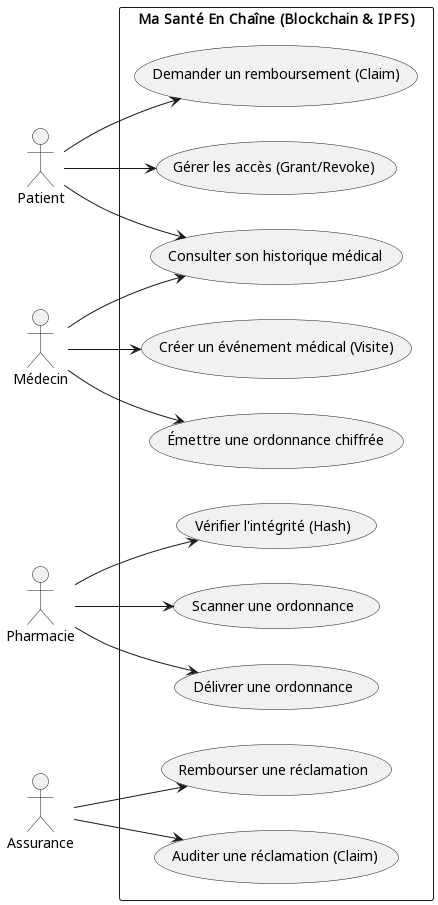
\includegraphics[width=\textwidth]{diagramme_cas_utilisation.png}
    \caption{Diagramme global des cas d'utilisation de la plateforme}
    \label{fig:use_cases}
\end{figure}

\textbf{Le diagramme ci-dessus indique que :}

Le \textbf{Patient} est au centre du système. Il consulte son historique médical immuable, gère finement ses droits d'accès (Grant/Revoke), et soumet des demandes de remboursement (Claims) à son assurance. Ces actions sont directement exécutées sur le Smart Contract via des transactions signées par son Wallet.

Le \textbf{Médecin} est l'autorité prescriptrice. Ses responsabilités incluent la création d'événements médicaux (visites, diagnostics) et l'émission d'ordonnances chiffrées. Chaque acte est signé cryptographiquement, chiffré via AES-GCM, envoyé sur IPFS, et ancré sur la blockchain.

La \textbf{Pharmacie} agit comme un point de validation critique. Elle scanne les ordonnances, vérifie mathématiquement l'intégrité des documents via la comparaison des Hashs SHA-256, et verrouille définitivement l'ordonnance sur le registre en changeant son statut en \texttt{DELIVERED}.

L'\textbf{Assurance} est le moteur d'audit. Elle vérifie les preuves cryptographiques associées aux Claims et émet des décisions de remboursement traçables sur la blockchain.

\subsection{Diagrammes de Séquence}
Un diagramme de séquence décrit comment les objets et les composants d'un système interagissent entre eux au fil du temps. Il met en évidence l'ordre chronologique des messages échangés et montre comment les interactions se déroulent étape par étape. Ce type de diagramme est essentiel pour comprendre le comportement dynamique du système et analyser les flux de communication.

\subsubsection{Diagramme de Séquence : Émission d'une Ordonnance}
\begin{figure}[H]
    \centering
    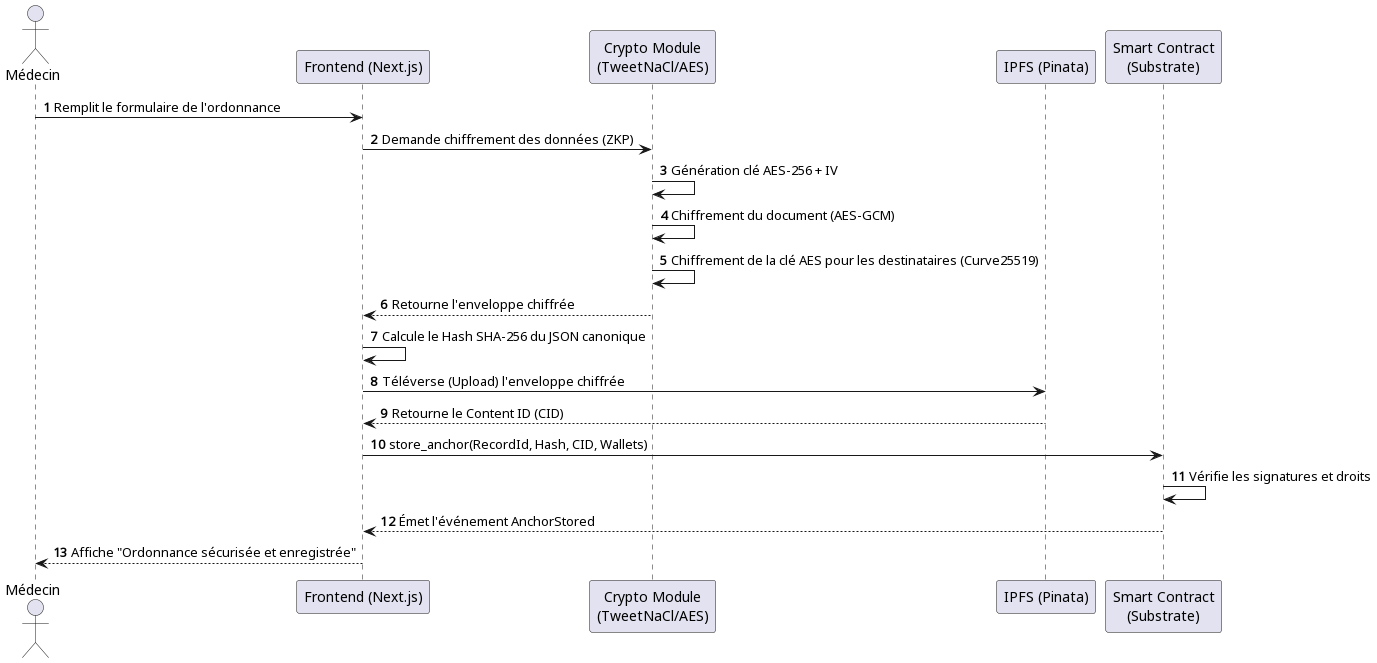
\includegraphics[width=\textwidth]{diagramme_sequence.png}
    \caption{Diagramme de Séquence : Émission et Ancrage d'une Ordonnance}
    \label{fig:seq_prescription}
\end{figure}

\textbf{Le diagramme ci-dessus indique :}
\begin{enumerate}
    \item Le médecin remplit le formulaire de prescription dans le Frontend Next.js.
    \item Le module cryptographique génère une clé AES-256 aléatoire et un IV de 12 octets.
    \item Le document JSON est canonisé (tri alphabétique des clés) puis chiffré en AES-GCM.
    \item La clé AES est chiffrée pour chaque destinataire (patient, pharmacie) via des boîtes NaCl (Curve25519).
    \item L'enveloppe chiffrée est téléversée sur IPFS/Pinata, générant un CID unique.
    \item Le Frontend forge une transaction \texttt{store\_anchor} contenant le RecordId, le Hash SHA-256, le CID, et les Wallets autorisés.
    \item Le Smart Contract vérifie la signature et émet l'événement \texttt{AnchorStored}.
\end{enumerate}

\subsubsection{Diagramme de Séquence : Vérification et Délivrance Pharmacie}
\begin{figure}[H]
    \centering
    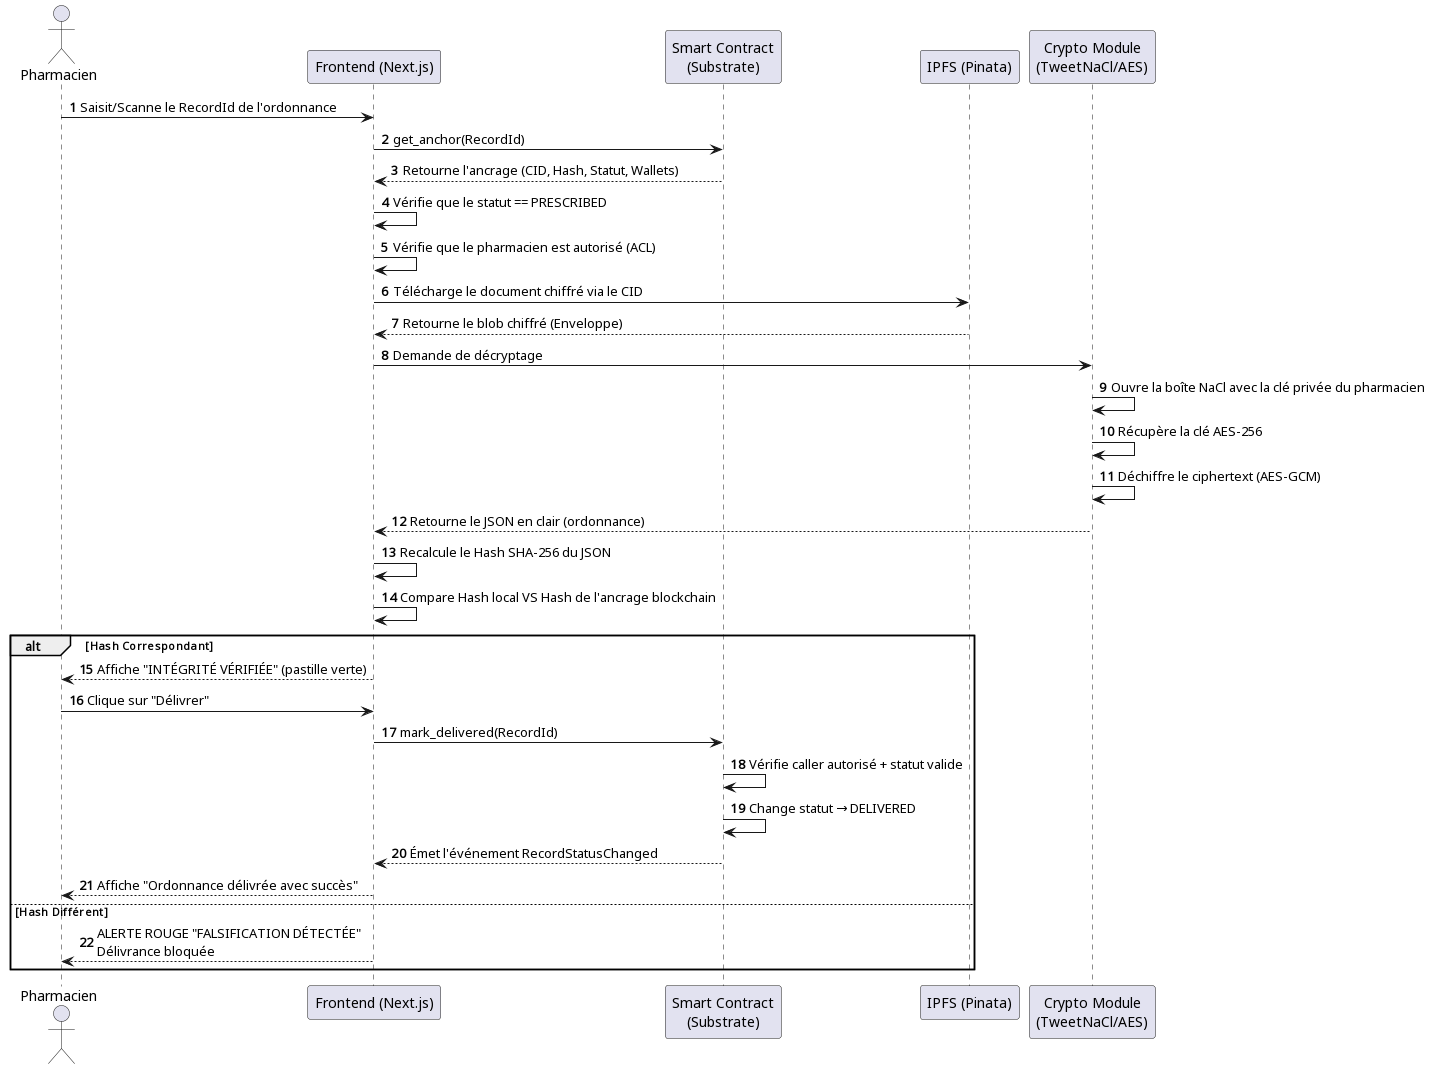
\includegraphics[width=\textwidth]{diagramme_sequence_pharmacie.png}
    \caption{Diagramme de Séquence : Pipeline de Vérification et Délivrance par la Pharmacie}
    \label{fig:seq_pharmacy}
\end{figure}

\textbf{Le diagramme ci-dessus indique :}
\begin{enumerate}
    \item Le pharmacien saisit ou scanne le RecordId.
    \item Le système interroge le Smart Contract (\texttt{get\_anchor}) pour récupérer le CID, le Hash, le statut et les Wallets autorisés.
    \item Le Frontend vérifie que le statut est \texttt{PRESCRIBED} et que le pharmacien est dans l'ACL.
    \item Le document chiffré est téléchargé depuis IPFS via le CID.
    \item La boîte NaCl du pharmacien est ouverte avec sa clé privée pour récupérer la clé AES.
    \item Le ciphertext est déchiffré en AES-GCM, reconstituant le JSON de l'ordonnance.
    \item \textbf{Étape critique :} Le Hash SHA-256 est recalculé localement et comparé avec celui stocké on-chain.
    \item Si les hashs correspondent : intégrité vérifiée, la délivrance est autorisée. Si les hashs divergent : \textbf{ALERTE FALSIFICATION}, la délivrance est bloquée.
\end{enumerate}

\subsubsection{Diagramme de Séquence : Pipeline Assurance (Claims)}
\begin{figure}[H]
    \centering
    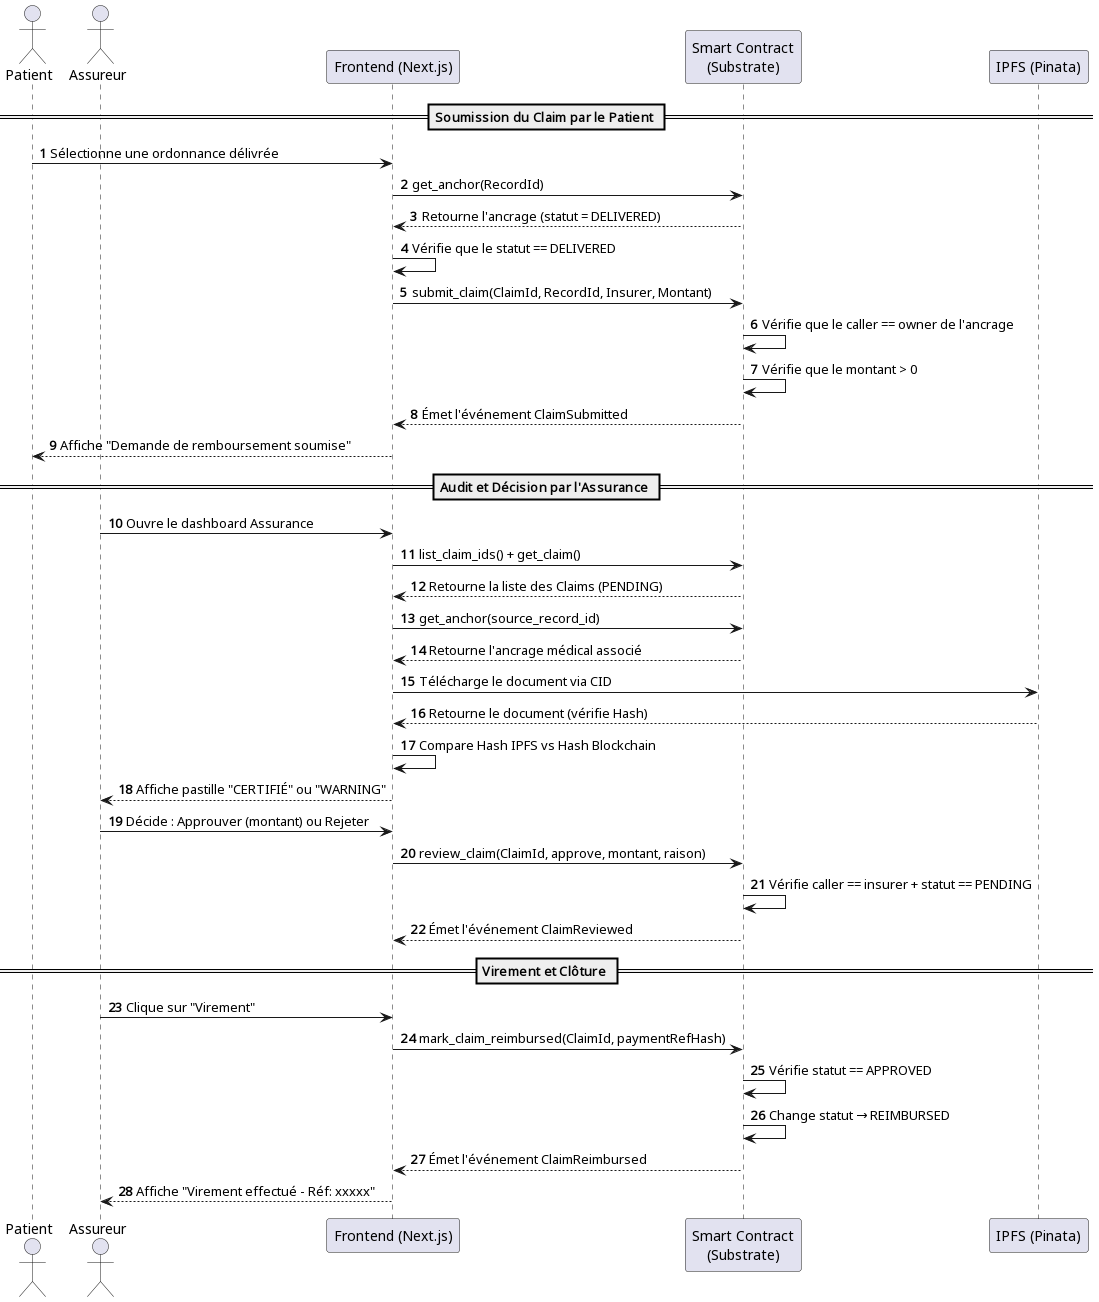
\includegraphics[width=\textwidth]{diagramme_sequence_assurance.png}
    \caption{Diagramme de Séquence : Pipeline de Soumission, Audit et Remboursement}
    \label{fig:seq_assurance}
\end{figure}

\subsection{Modélisation des Données On-Chain (Smart Contract ink!)}
Contrairement aux bases de données relationnelles (SQL) ou documentaires (MongoDB), le stockage on-chain est extrêmement coûteux. Nous avons donc conçu des structures de données minimalistes en Rust :

\begin{table}[H]
    \centering
    \caption{Structures de données stockées on-chain dans le Smart Contract}
    \label{tab:structures_onchain}
    \begin{tabular}{|p{3.5cm}|p{10cm}|}
        \hline
        \textbf{Structure} & \textbf{Champs principaux} \\
        \hline
        \texttt{Anchor} & \texttt{kind} (Prescription/Visit/LabResult/Operation), \texttt{cid} (bytes IPFS), \texttt{data\_hash} (SHA-256 32 bytes), \texttt{owner}, \texttt{doctor}, \texttt{pharmacy?}, \texttt{insurer?}, \texttt{status} (Prescribed/Delivered/Cancelled), \texttt{created\_at}, \texttt{updated\_at} \\
        \hline
        \texttt{Claim} & \texttt{source\_record\_id}, \texttt{claimant}, \texttt{insurer}, \texttt{amount\_requested}, \texttt{amount\_approved?}, \texttt{status} (Pending/Approved/Rejected/Reimbursed), \texttt{reason\_hash?}, \texttt{payment\_ref\_hash?}, timestamps \\
        \hline
        \texttt{Mappings} & \texttt{records: Mapping<RecordId, Anchor>}, \texttt{claims: Mapping<ClaimId, Claim>}, \texttt{access: Mapping<(RecordId, AccountId), bool>}, \texttt{encryption\_keys: Mapping<AccountId, [u8;32]>} \\
        \hline
    \end{tabular}
\end{table}

\subsection{Machine à États}
Les transitions d'état sont strictement contrôlées par le Smart Contract. Aucune transition invalide ne peut être exécutée :

\textbf{Cycle de vie d'une Ordonnance :}
\begin{itemize}
    \item \texttt{PRESCRIBED} $\rightarrow$ \texttt{DELIVERED} (par la pharmacie autorisée)
    \item \texttt{PRESCRIBED} $\rightarrow$ \texttt{CANCELLED} (par le médecin ou le patient)
    \item \texttt{DELIVERED} $\rightarrow$ toute transition : \textbf{BLOQUÉE}
    \item \texttt{CANCELLED} $\rightarrow$ toute transition : \textbf{BLOQUÉE}
\end{itemize}

\textbf{Cycle de vie d'un Claim :}
\begin{itemize}
    \item \texttt{PENDING} $\rightarrow$ \texttt{APPROVED} / \texttt{REJECTED} (par l'assureur)
    \item \texttt{APPROVED} $\rightarrow$ \texttt{REIMBURSED} (par l'assureur après virement)
    \item \texttt{REJECTED} $\rightarrow$ toute transition : \textbf{BLOQUÉE}
    \item \texttt{REIMBURSED} $\rightarrow$ toute transition : \textbf{BLOQUÉE}
\end{itemize}

\section{Conclusion}
Ce chapitre d'analyse et conception nous a permis de définir avec précision les bases de notre système décentralisé. La spécification des acteurs, des cas d'utilisation et la création des diagrammes UML établissent une compréhension claire des fonctionnalités attendues et des interactions sécurisées entre les acteurs et le Smart Contract. Ces éléments constituent le socle de la phase de réalisation détaillée dans les chapitres suivants.
% =======================================================
% CHAPITRE 3 : TECHNOLOGIES ET OUTILS
% =======================================================
\chapter{Technologies et Outils Utilisés}

\section{Introduction}
Dans ce chapitre, nous détaillons les différentes technologies et outils utilisés dans le développement de « Ma Santé En Chaîne ». Chaque technologie a été sélectionnée en fonction de ses avantages spécifiques pour la construction d'une application décentralisée sécurisée et performante.

\section{Technologies}

\subsection{Technologies utilisées pour la couche Blockchain (Back-end décentralisé)}

\begin{table}[H]
    \centering
    \caption{Technologies de la couche Blockchain}
    \label{tab:tech_blockchain}
    \begin{tabular}{|p{3.5cm}|p{10cm}|}
        \hline
        \textbf{Technologie} & \textbf{Description et rôle dans le projet} \\
        \hline
        \textbf{Rust} & Langage de programmation système développé par Mozilla, offrant des garanties de sécurité mémoire sans ramasse-miettes (garbage collector). Dans notre projet, Rust est utilisé pour l'écriture du Smart Contract, bénéficiant de son système de typage strict qui élimine par design des classes entières de vulnérabilités (buffer overflow, data races). \\
        \hline
        \textbf{Substrate} & Framework modulaire open-source développé par Parity Technologies (créateurs de Polkadot). Il permet de construire des blockchains personnalisées avec un consensus configurable. Nous utilisons \texttt{substrate-contracts-node} comme environnement d'exécution local avec stockage persistant dans le dossier \texttt{blockchain-data/}. \\
        \hline
        \textbf{ink!} & eDSL (Embedded Domain Specific Language) de l'écosystème Polkadot pour l'écriture de Smart Contracts. Contrairement à Solidity (Ethereum), ink! est compilé en WebAssembly (Wasm) natif, offrant des performances supérieures et la sécurité de typage de Rust. Les macros \texttt{\#[ink::contract]} et \texttt{\#[ink(message)]} simplifient la déclaration des fonctions publiques du contrat. \\
        \hline
        \textbf{WebAssembly (Wasm)} & Format d'instruction binaire portable servant de cible de compilation pour les contrats ink!. Le fichier \texttt{.wasm} généré est déployé sur le nœud Substrate et exécuté dans un environnement sandboxé et sécurisé. \\
        \hline
    \end{tabular}
\end{table}

\subsection{Technologies utilisées pour le stockage décentralisé}

\begin{table}[H]
    \centering
    \caption{Technologies de stockage décentralisé}
    \label{tab:tech_storage}
    \begin{tabular}{|p{3.5cm}|p{10cm}|}
        \hline
        \textbf{Technologie} & \textbf{Description et rôle dans le projet} \\
        \hline
        \textbf{IPFS} & InterPlanetary File System. Au lieu de localiser un fichier par son emplacement physique (URL), IPFS le localise par son contenu (Content Addressing) via son CID. Si un seul octet du fichier médical change, le CID change complètement, garantissant l'intégrité par design. \\
        \hline
        \textbf{Pinata} & Service de « pinning » IPFS garantissant que nos fichiers restent en permanence disponibles et répliqués sur le réseau mondial, même si le client d'origine se déconnecte. Pinata expose une API REST sécurisée par JWT pour l'upload et le téléchargement de fichiers. \\
        \hline
    \end{tabular}
\end{table}

\subsection{Technologies utilisées pour le développement Frontend}

\begin{table}[H]
    \centering
    \caption{Technologies Frontend}
    \label{tab:tech_frontend}
    \begin{tabular}{|p{3.5cm}|p{10cm}|}
        \hline
        \textbf{Technologie} & \textbf{Description et rôle dans le projet} \\
        \hline
        \textbf{Next.js 14} & Framework React de référence avec App Router. Il sert de moteur d'orchestration global. Bien qu'il n'y ait pas de base de données backend traditionnelle, les API Routes (Edge) servent de proxys légers pour contourner les restrictions CORS des passerelles IPFS. \\
        \hline
        \textbf{React 18} & Bibliothèque JavaScript pour la construction d'interfaces utilisateur dynamiques et réactives. Les composants React gèrent les états complexes de chaque dashboard (chargement, transactions en cours, vérification d'intégrité). \\
        \hline
        \textbf{Tailwind CSS} & Framework utilitaire CSS permettant de concevoir rapidement des interfaces modernes. Notre UI adopte un thème « Dark Mode » avec des effets de Glassmorphism et une typographie monospace évoquant l'univers blockchain. \\
        \hline
        \textbf{TypeScript} & Sur-ensemble typé de JavaScript. L'ensemble du code frontend est écrit en TypeScript, apportant une vérification de types à la compilation et réduisant les erreurs à l'exécution. \\
        \hline
    \end{tabular}
\end{table}

\subsection{Technologies utilisées pour la couche cryptographique}

\begin{table}[H]
    \centering
    \caption{Technologies cryptographiques}
    \label{tab:tech_crypto}
    \begin{tabular}{|p{3.5cm}|p{10cm}|}
        \hline
        \textbf{Technologie} & \textbf{Description et rôle dans le projet} \\
        \hline
        \textbf{Polkadot.js API} & Interface de programmation permettant au navigateur de communiquer via WebSockets (RPC) avec le nœud Substrate. Elle gère l'estimation des frais de Gas, l'injection de la signature utilisateur, et le décodage des événements du contrat. \\
        \hline
        \textbf{TweetNaCl.js} & Implémentation JavaScript auditée de la bibliothèque cryptographique NaCl (Networking and Cryptography library). Elle fournit les primitives pour le chiffrement asymétrique Curve25519/XSalsa20/Poly1305 utilisées dans notre schéma d'enveloppe hybride. \\
        \hline
        \textbf{Web Crypto API} & API native du navigateur pour les opérations cryptographiques (AES-GCM, SHA-256, PBKDF2). Disponible uniquement dans un contexte sécurisé (HTTPS ou localhost). \\
        \hline
    \end{tabular}
\end{table}

\section{Outils de Développement}

\begin{table}[H]
    \centering
    \caption{Outils de développement utilisés}
    \label{tab:outils}
    \begin{tabular}{|p{3.5cm}|p{10cm}|}
        \hline
        \textbf{Outil} & \textbf{Utilisation dans le projet} \\
        \hline
        \textbf{VS Code} & Éditeur de code principal avec extensions Rust-Analyzer et ink! pour le développement du Smart Contract, et ESLint/Prettier pour le code TypeScript. \\
        \hline
        \textbf{cargo-contract} & CLI officiel pour compiler, tester et déployer les contrats ink! sur Substrate. Commande de build : \texttt{cargo contract build --release}. \\
        \hline
        \textbf{Polkadot.js Apps} & Interface web pour interagir manuellement avec le nœud Substrate, inspecter les blocs, et debugger les transactions. \\
        \hline
        \textbf{Git / GitHub} & Système de contrôle de version distribué pour la gestion du code source et la collaboration d'équipe. \\
        \hline
        \textbf{PlantUML} & Outil de génération de diagrammes UML à partir de descriptions textuelles, utilisé pour produire les diagrammes de ce rapport. \\
        \hline
    \end{tabular}
\end{table}

\section{Conclusion}
Ce chapitre a présenté l'arsenal technologique complet déployé pour la réalisation de « Ma Santé En Chaîne ». La combinaison de Rust/ink! pour la sécurité du contrat, IPFS pour le stockage distribué, et Next.js/React pour l'expérience utilisateur constitue l'état de l'art du développement d'applications décentralisées (dApps). Le chapitre suivant détaillera la réalisation technique et le fonctionnement interne de chaque composant.

% =======================================================
% CHAPITRE 4 : REALISATION ET FONCTIONNEMENT DETAILLE
% =======================================================
\chapter{Réalisation et Fonctionnement Détaillé}

\section{Introduction}
Ce chapitre, cœur du rapport, plonge dans l'implémentation technique de « Ma Santé En Chaîne ». Il détaille l'architecture Web3 déployée, les pipelines cryptographiques internes, le fonctionnement de chaque tableau de bord, et les défis techniques rencontrés.

\section{Architecture Technique Globale}
L'architecture du projet repose sur trois couches distinctes, sans aucun serveur backend traditionnel :

\begin{enumerate}
    \item \textbf{Couche Présentation (Next.js)} : Interface utilisateur React avec sept dashboards spécialisés. Orchestre les appels cryptographiques et les transactions blockchain.
    \item \textbf{Couche Logique Métier (Smart Contract ink!)} : Contrat intelligent déployé sur Substrate. Gère les ancrages (\texttt{Anchor}), les claims, les transitions d'état et la matrice ACL.
    \item \textbf{Couche Stockage (IPFS/Pinata)} : Héberge les documents médicaux chiffrés. Le contrat ne stocke que les pointeurs (CID) et les empreintes (Hash SHA-256).
\end{enumerate}

\section{Mécanique de Chiffrement Hybride (Zero-Knowledge)}
Le plus grand défi technique est le respect du secret médical sur un réseau public. Le module \texttt{medicalCrypto.ts} implémente une architecture d'enveloppe hybride (\texttt{msce-hybrid-aesgcm-v2}).

\textbf{Processus de chiffrement détaillé :}
\begin{enumerate}
    \item \textbf{Génération de la clé symétrique :} Le navigateur génère une clé AES-256 aléatoire et un vecteur d'initialisation (IV) de 12 octets via \texttt{crypto.getRandomValues()}.
    \item \textbf{Canonisation JSON :} L'objet JSON est canonisé (tri alphabétique récursif des clés) pour garantir le déterminisme mathématique du hachage, indépendamment de l'ordre d'insertion des propriétés.
    \item \textbf{Chiffrement AES-GCM :} Le JSON canonisé est converti en octets puis chiffré via \texttt{crypto.subtle.encrypt()} avec l'algorithme AES-GCM (Galois/Counter Mode), produisant le \textit{ciphertext} et un tag d'authentification intégré.
    \item \textbf{Récupération des clés publiques :} Le système interroge le Smart Contract via \texttt{encryption\_key\_of(walletAddress)} pour obtenir les clés publiques Curve25519 de chaque destinataire.
    \item \textbf{Enveloppes NaCl :} Pour chaque destinataire, la clé AES est chiffrée dans une « boîte » NaCl utilisant l'échange de clés X25519, le chiffrement XSalsa20 et le MAC Poly1305. Un nonce éphémère unique est généré par boîte.
    \item \textbf{Construction de l'enveloppe finale :} L'objet JSON envoyé sur IPFS contient : \texttt{version}, \texttt{algorithm}, \texttt{ivB64}, \texttt{ciphertextB64}, \texttt{payloadHashHex}, et un tableau \texttt{encryptedKeys[]} (une entrée par destinataire avec \texttt{walletAddress}, \texttt{senderPublicKeyHex}, \texttt{nonceB64}, \texttt{encryptedDataKeyB64}).
\end{enumerate}

Le \textbf{décryptage} suit le chemin inverse : le destinataire ouvre sa boîte NaCl avec sa clé privée, récupère la clé AES en RAM, déchiffre le ciphertext, et accède au contenu médical. À aucun moment la clé privée ou le document en clair ne quitte le navigateur.

\section{Données On-Chain vs Off-Chain}
\begin{table}[H]
    \centering
    \caption{Répartition des données entre Blockchain et IPFS}
    \label{tab:onchain_offchain}
    \begin{tabular}{|p{6.5cm}|p{6.5cm}|}
        \hline
        \textbf{Stocké sur la Blockchain (On-Chain)} & \textbf{Stocké sur IPFS (Off-Chain)} \\
        \hline
        Identifiants (RecordId, ClaimId) & Ordonnances chiffrées (schema \texttt{msce-prescription-v2}) \\
        \hline
        Empreintes SHA-256 (32 bytes) & Événements médicaux (visites, analyses) \\
        \hline
        Pointeurs CID vers IPFS & Tickets de délivrance pharmacie \\
        \hline
        Statuts (Prescribed, Delivered...) & Documents gouvernance (rôles, identités) \\
        \hline
        Wallets autorisés (owner, doctor...) & Profils utilisateur \\
        \hline
        Clés publiques de chiffrement (32 bytes) & PDF encodés en base64 dans JSON \\
        \hline
        Horodatages de création/modification & --- \\
        \hline
    \end{tabular}
\end{table}

\section{Pipeline d'Authentification « Wallet-First »}
Le processus de connexion s'affranchit totalement du couple classique email/mot de passe :
\begin{enumerate}
    \item L'utilisateur clique sur « Se Connecter ». L'extension Polkadot.js du navigateur intercepte la demande.
    \item Le module \texttt{wallet.ts} appelle \texttt{getExtension().enable("Ma Sante en Chaine")} pour obtenir l'accès aux comptes.
    \item Le premier compte Wallet disponible est sélectionné. Son adresse publique devient l'identité de l'utilisateur.
    \item Le système interroge les ancrages de gouvernance sur la blockchain et IPFS (\texttt{resolveWalletRoleOnChain}) pour déterminer le rôle de cette adresse (Médecin, Pharmacien, Patient, etc.).
    \item Une session locale est créée et stockée dans \texttt{localStorage} avec le token JWT simulé, le rôle résolu et les métadonnées d'identité.
    \item L'utilisateur est redirigé vers le dashboard correspondant à son rôle.
\end{enumerate}

\section{Présentation des Dashboards}

\subsection{Accès à l'application}
La page d'authentification est une interface sécurisée Wallet-First qui vérifie l'identité de l'utilisateur via sa signature cryptographique. Contrairement aux systèmes traditionnels, aucun mot de passe n'est requis. L'identité est prouvée mathématiquement par la possession de la clé privée associée au portefeuille.

\subsection{Dashboard Médecin}
Le tableau de bord du médecin est le point d'entrée principal pour la création d'actes médicaux.

\textbf{Fonctionnement en arrière-plan lors d'une prescription :}
\begin{enumerate}
    \item Les données du formulaire (médicaments, posologie, instructions) sont agrégées en un objet JSON.
    \item Le pipeline de chiffrement hybride est déclenché (\texttt{encryptMedicalPayloadOrPlain}).
    \item Si les clés publiques des destinataires sont disponibles on-chain, le chiffrement AES-GCM + NaCl est appliqué. Sinon, un mode dégradé (\texttt{PLAIN\_IPFS\_FALLBACK}) est utilisé avec un avertissement.
    \item L'enveloppe chiffrée est envoyée à l'API Pinata (\texttt{uploadJsonToIpfs}) avec un mécanisme de retry exponentiel (\texttt{withUploadRetry}).
    \item Le CID retourné par Pinata est utilisé pour forger la transaction \texttt{store\_anchor} sur le Smart Contract, incluant le RecordId (hash Blake2 de la clé logique), le Hash SHA-256 du payload, et les adresses des Wallets autorisés.
    \item Un Dry Run (simulation) est exécuté avant la signature pour vérifier que le contrat ne rejettera pas la transaction.
    \item L'utilisateur signe la transaction via l'extension Polkadot.js.
    \item Une fois le bloc miné, l'interface est notifiée via WebSocket et l'ordonnance apparaît dans la liste.
\end{enumerate}

\begin{figure}[H]
    \centering
    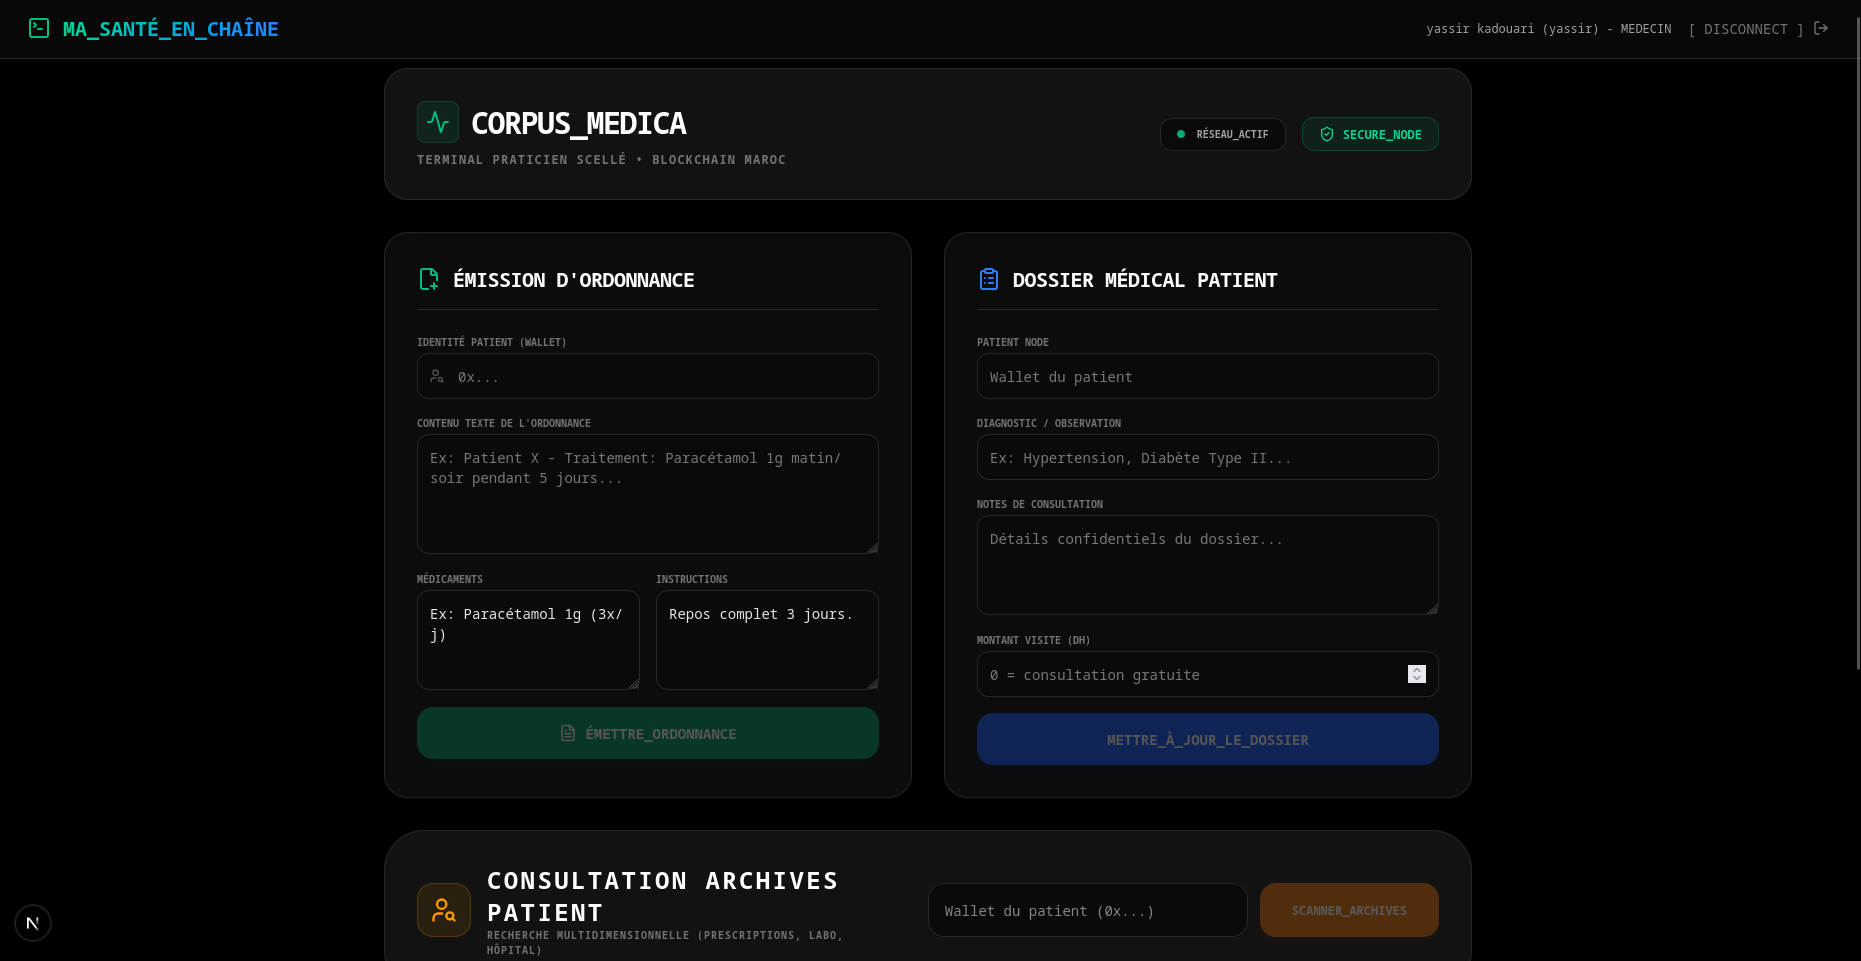
\includegraphics[width=\textwidth]{screenshots/medecin/dashboard.png}
    \caption{Tableau de bord Médecin : Interface de Prescription Décentralisée}
    \label{fig:dash_medecin}
\end{figure}

\subsection{Dashboard Pharmacie}
L'interface de la pharmacie est conçue comme un scanner et un point de validation critique de la chaîne de confiance.

\textbf{Mécanique de vérification et délivrance :}
\begin{enumerate}
    \item Le pharmacien saisit ou scanne le QR Code contenant le \texttt{RecordId}. Le système normalise l'entrée via \texttt{normalizeAnchorLookupInput()} qui supporte les URLs, les préfixes \texttt{msc:prescription:}, et les hashs hexadécimaux.
    \item Le Smart Contract est interrogé (\texttt{get\_anchor}) : l'ordonnance est-elle valide (\texttt{Prescribed}) ? Le pharmacien est-il dans l'ACL ?
    \item Le document chiffré est téléchargé depuis IPFS via le CID.
    \item La boîte NaCl du pharmacien est ouverte, la clé AES est récupérée, et le document JSON est reconstitué.
    \item \textbf{Étape critique :} Le Hash SHA-256 est recalculé localement (\texttt{bodyDigest}) et comparé strictement avec celui stocké on-chain (\texttt{verifyHashOnChain}). Si un attaquant modifie le fichier sur IPFS, les hashs divergeront et l'interface affichera une alerte \textbf{« FALSIFICATION DÉTECTÉE »}, bloquant la délivrance.
    \item Si tout est conforme, le pharmacien clique sur « Délivrer ». La transaction \texttt{mark\_delivered} est forgée, verrouillant définitivement l'ordonnance.
    \item Un ticket de délivrance (\texttt{receipt:}) est créé et ancré séparément, contenant le montant total.
\end{enumerate}

\begin{figure}[H]
    \centering
    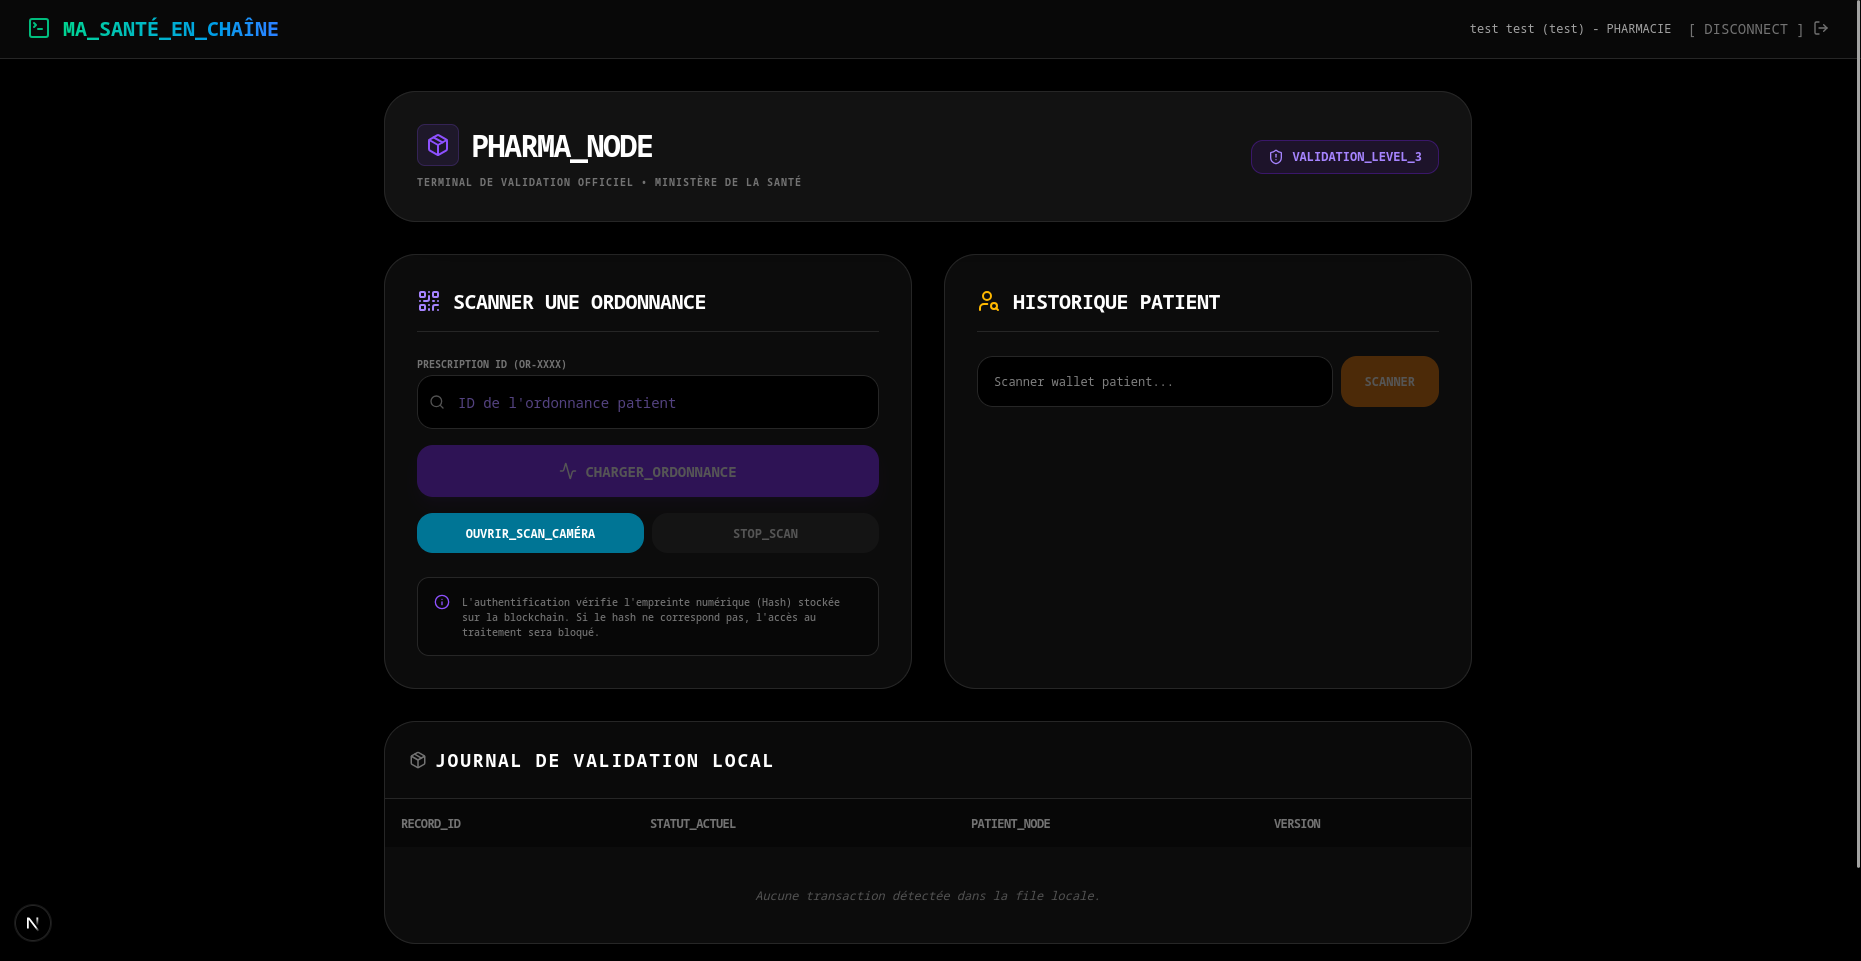
\includegraphics[width=\textwidth]{screenshots/pharmcaie/dashboard.png}
    \caption{Tableau de bord Pharmacie : Vue d'ensemble des ordonnances}
    \label{fig:dash_pharmacy}
\end{figure}

\begin{figure}[H]
    \centering
    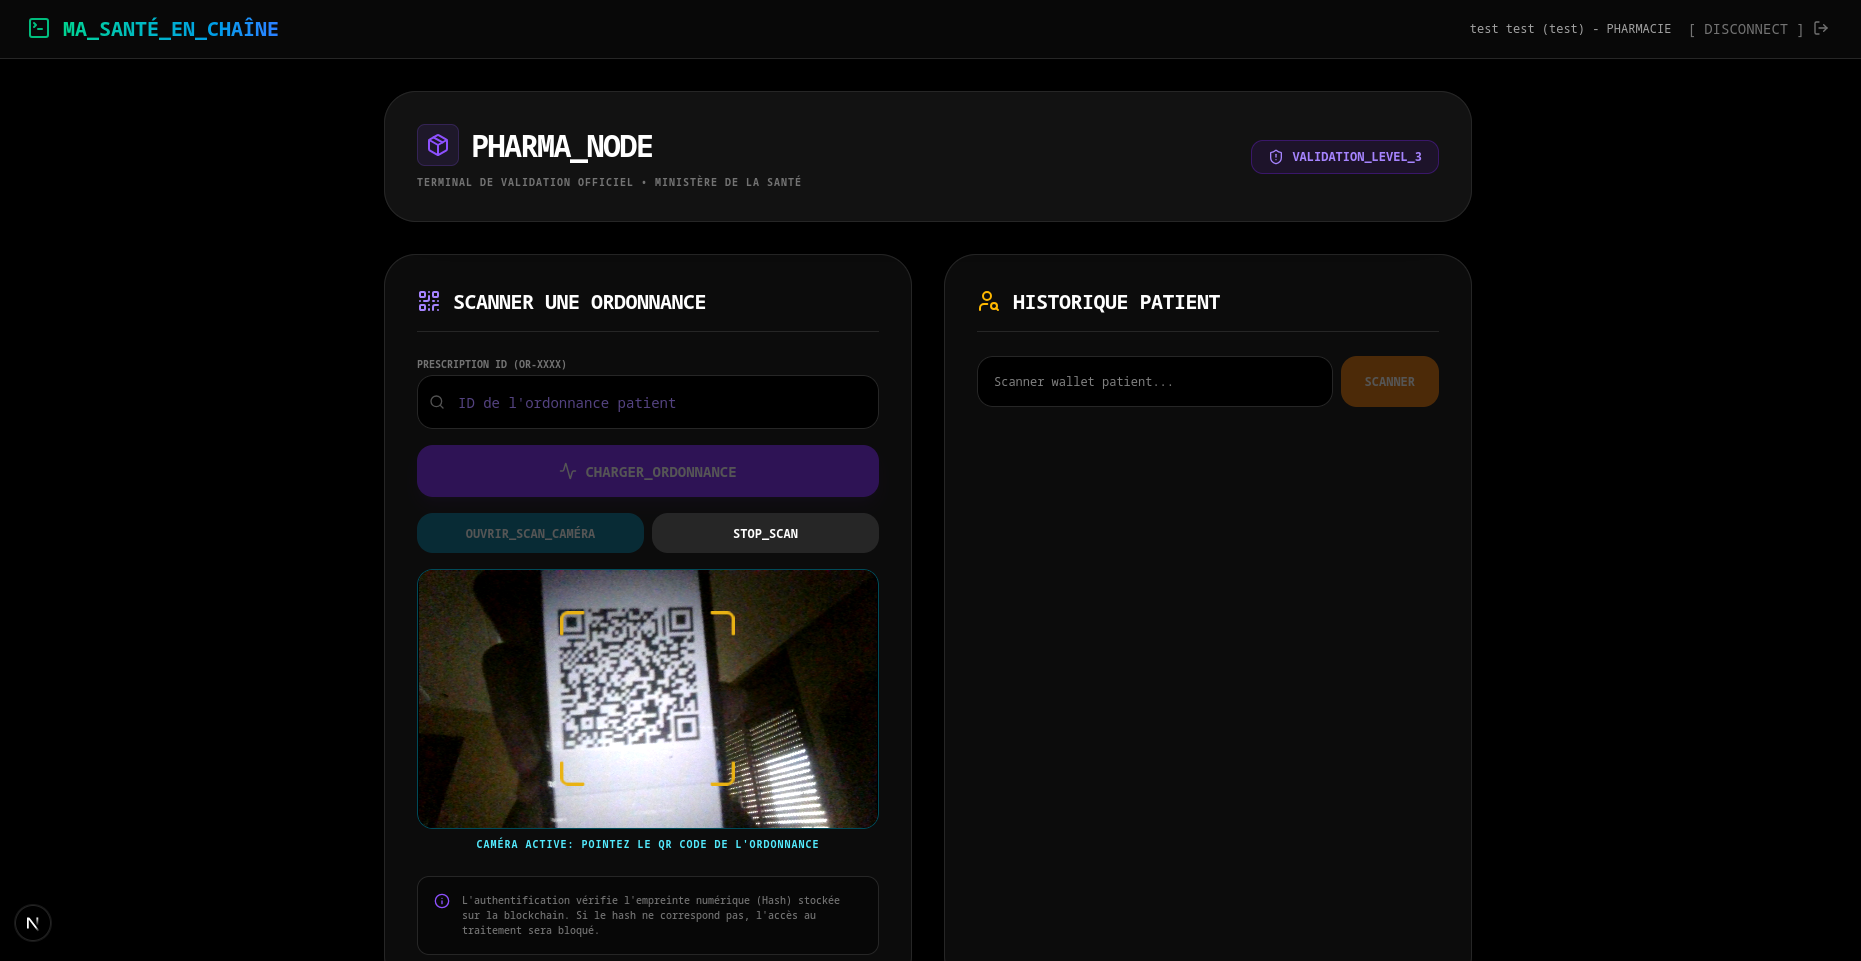
\includegraphics[width=\textwidth]{screenshots/pharmcaie/scanning qr code.png}
    \caption{Pharmacie : Scan du QR Code de l'ordonnance}
    \label{fig:dash_pharmacy_scan}
\end{figure}

\begin{figure}[H]
    \centering
    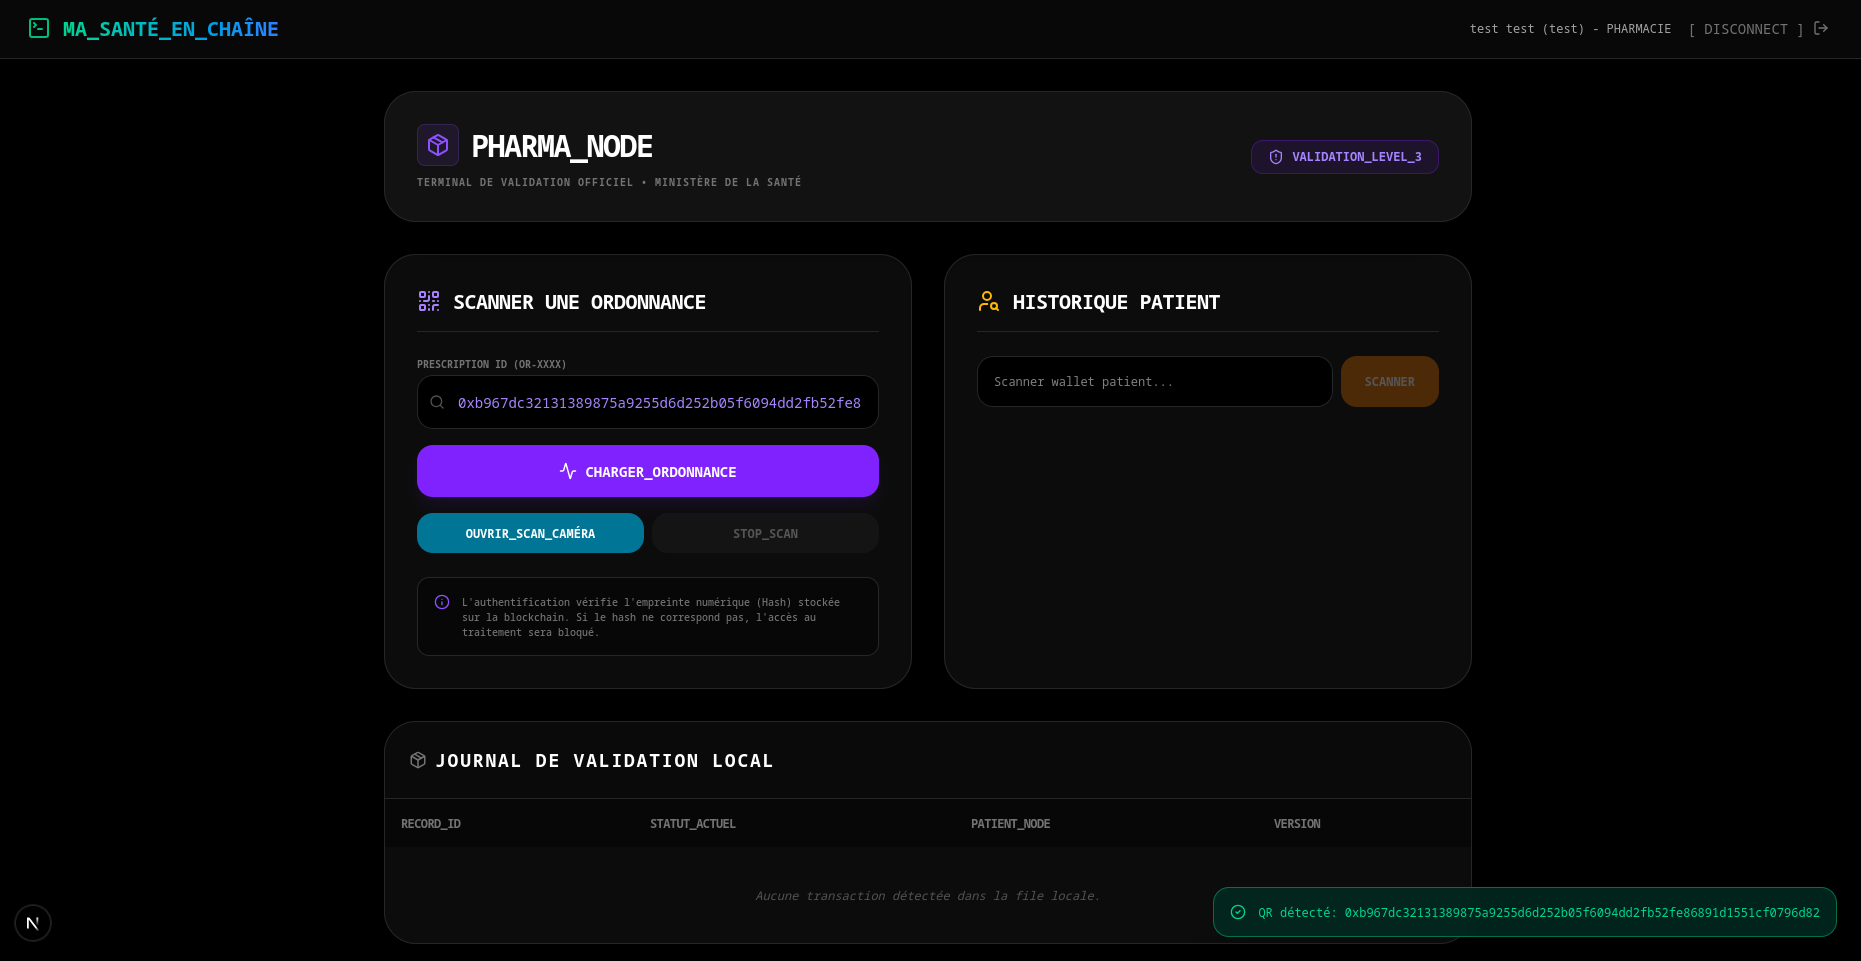
\includegraphics[width=\textwidth]{screenshots/pharmcaie/qr code scanned.png}
    \caption{Pharmacie : Résultat du scan et vérification d'intégrité blockchain}
    \label{fig:dash_pharmacy_scanned}
\end{figure}

\subsection{Dashboard Patient}
Le patient dispose d'une vue souveraine sur l'ensemble de son historique médical immuable.

\textbf{Fonctionnalités principales :}
\begin{itemize}
    \item Consultation de toutes les ordonnances (en cours et délivrées) liées à son Wallet.
    \item Gestion fine des droits d'accès : le patient peut accorder (\texttt{grant\_access}) ou révoquer (\texttt{revoke\_access}) l'accès de n'importe quel praticien à ses dossiers.
    \item Soumission de demandes de remboursement (Claims) : le patient sélectionne une ordonnance délivrée, spécifie le montant et l'assureur, et la transaction \texttt{submit\_claim} est envoyée au contrat.
    \item Configuration du profil médical : médecin traitant, groupe sanguin, pathologies, région.
\end{itemize}

\begin{figure}[H]
    \centering
    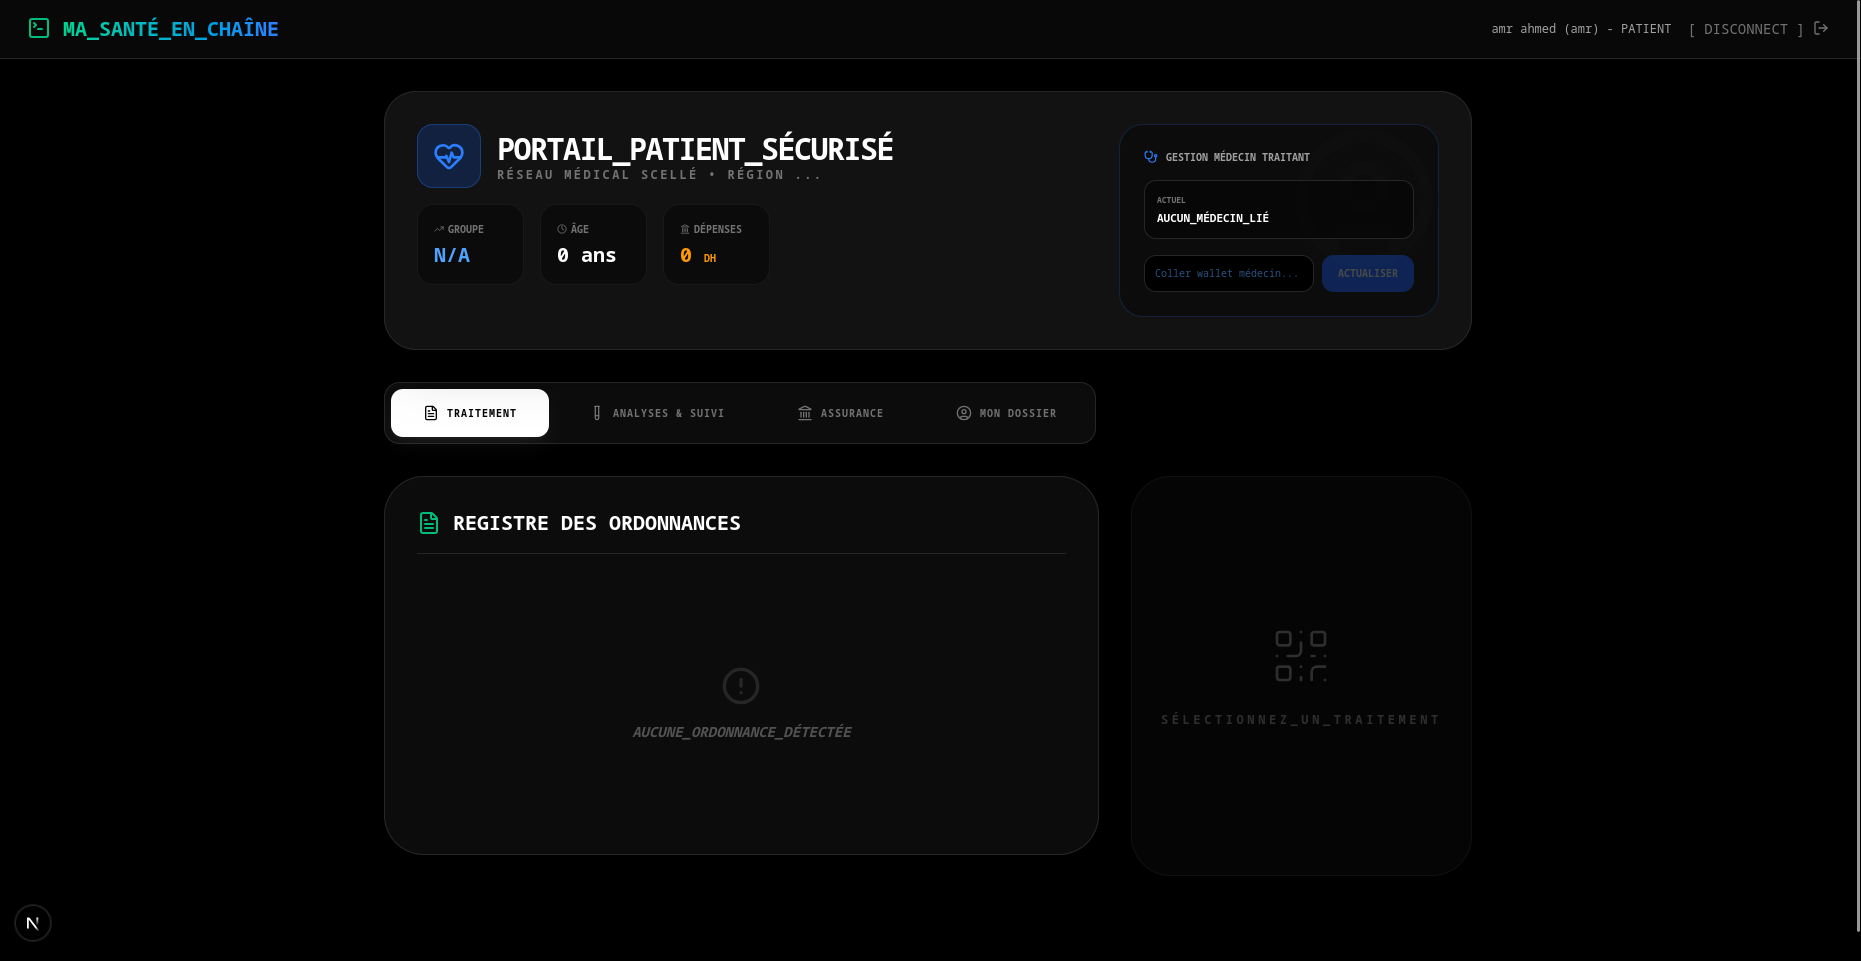
\includegraphics[width=\textwidth]{screenshots/patient/dashboard.png}
    \caption{Tableau de bord Patient : Historique médical et gestion des accès}
    \label{fig:dash_patient}
\end{figure}

\subsection{Dashboard Assurance (Insure\_Node)}
Le dashboard de l'assurance est un véritable moteur d'audit cryptographique.

\textbf{Fonctionnement du moteur de remboursement :}
\begin{enumerate}
    \item Le système liste les Claims via \texttt{listClaimsFromChain()} et filtre ceux adressés au Wallet de l'assureur connecté.
    \item Pour chaque Claim, le système récupère l'ancrage source (\texttt{get\_anchor(source\_record\_id)}), vérifie son statut (\texttt{DELIVERED}), et valide l'intégrité du document IPFS en comparant les hashs.
    \item Une pastille visuelle « CERTIFIÉ » (verte) ou « WARNING » (rouge) indique le résultat de la vérification.
    \item L'agent d'assurance peut approuver (avec montant ajusté et justification) ou rejeter la demande via \texttt{review\_claim}.
    \item Après le virement bancaire externe, l'agent clôture le cycle avec \texttt{mark\_claim\_reimbursed}, ancrant la référence de paiement (\texttt{paymentRefHash}) sur la blockchain.
\end{enumerate}

\begin{figure}[H]
    \centering
    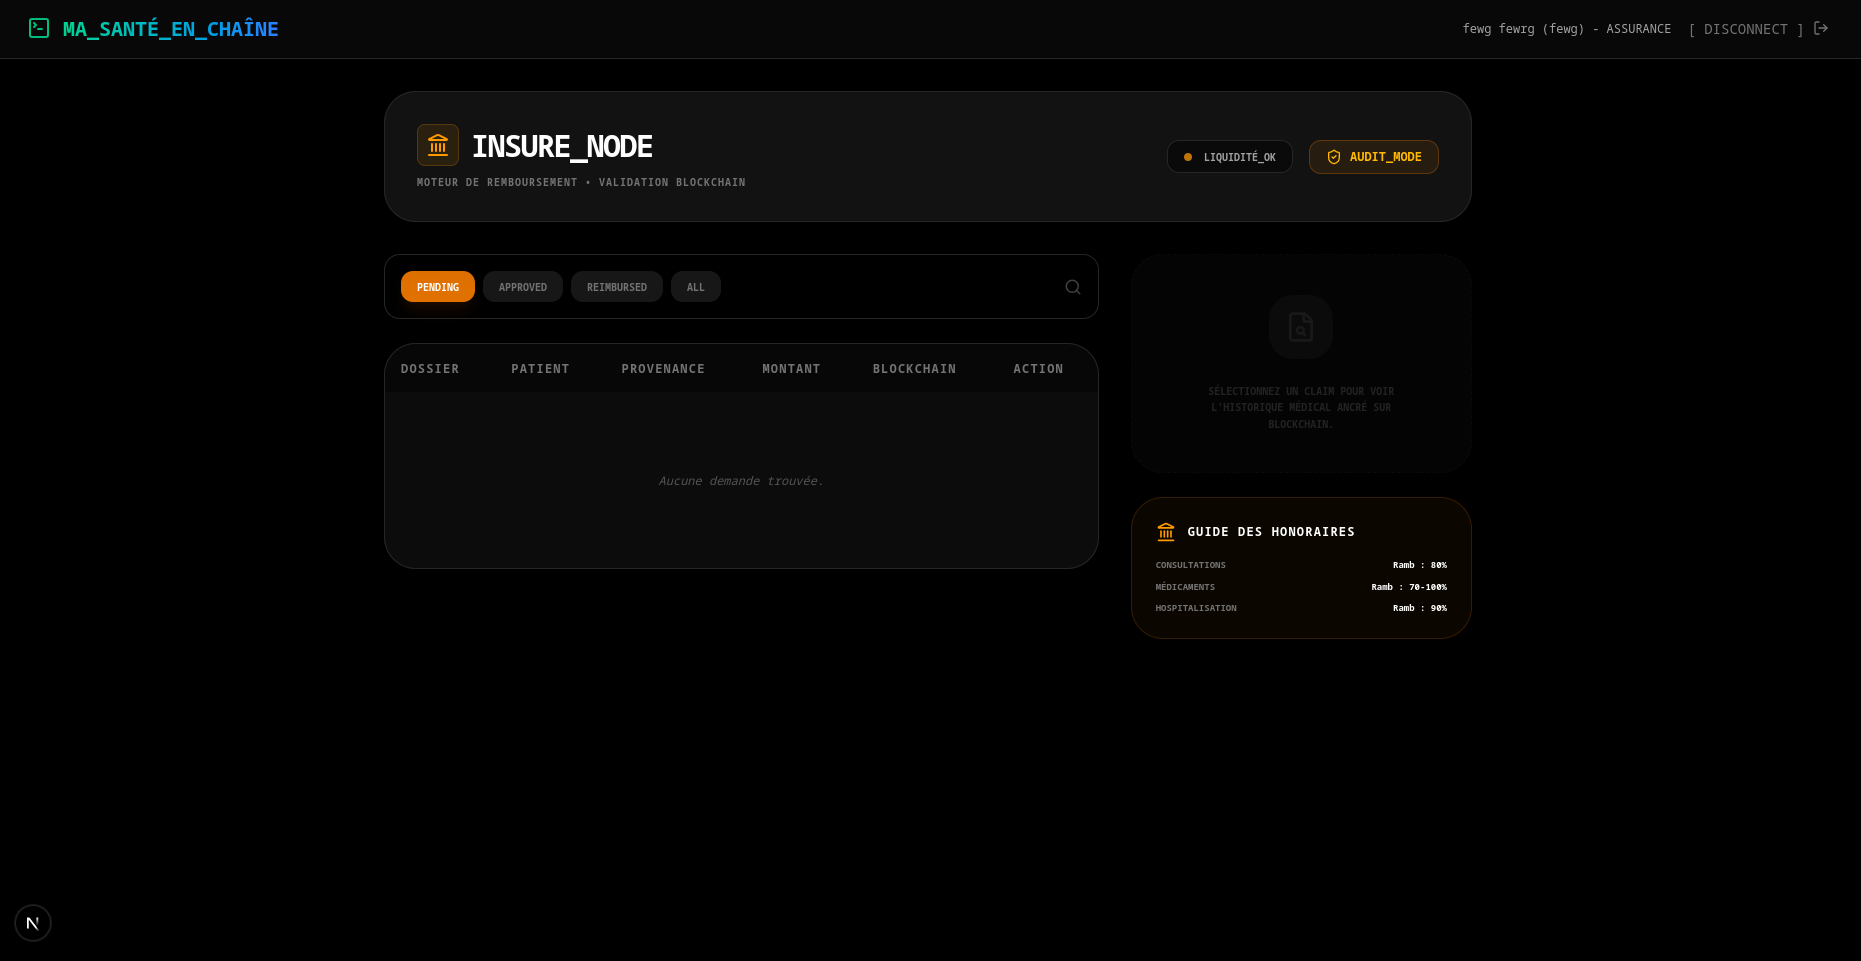
\includegraphics[width=\textwidth]{screenshots/assurance/Pasted image.png}
    \caption{Tableau de bord Assurance : Moteur d'audit et remboursement}
    \label{fig:dash_assurance}
\end{figure}

\subsection{Dashboard Laboratoire}
Le laboratoire peut soumettre des résultats d'analyses biologiques. Chaque résultat est ancré avec le type \texttt{LAB\_RESULT} et chiffré pour le patient et le médecin prescripteur.

\begin{figure}[H]
    \centering
    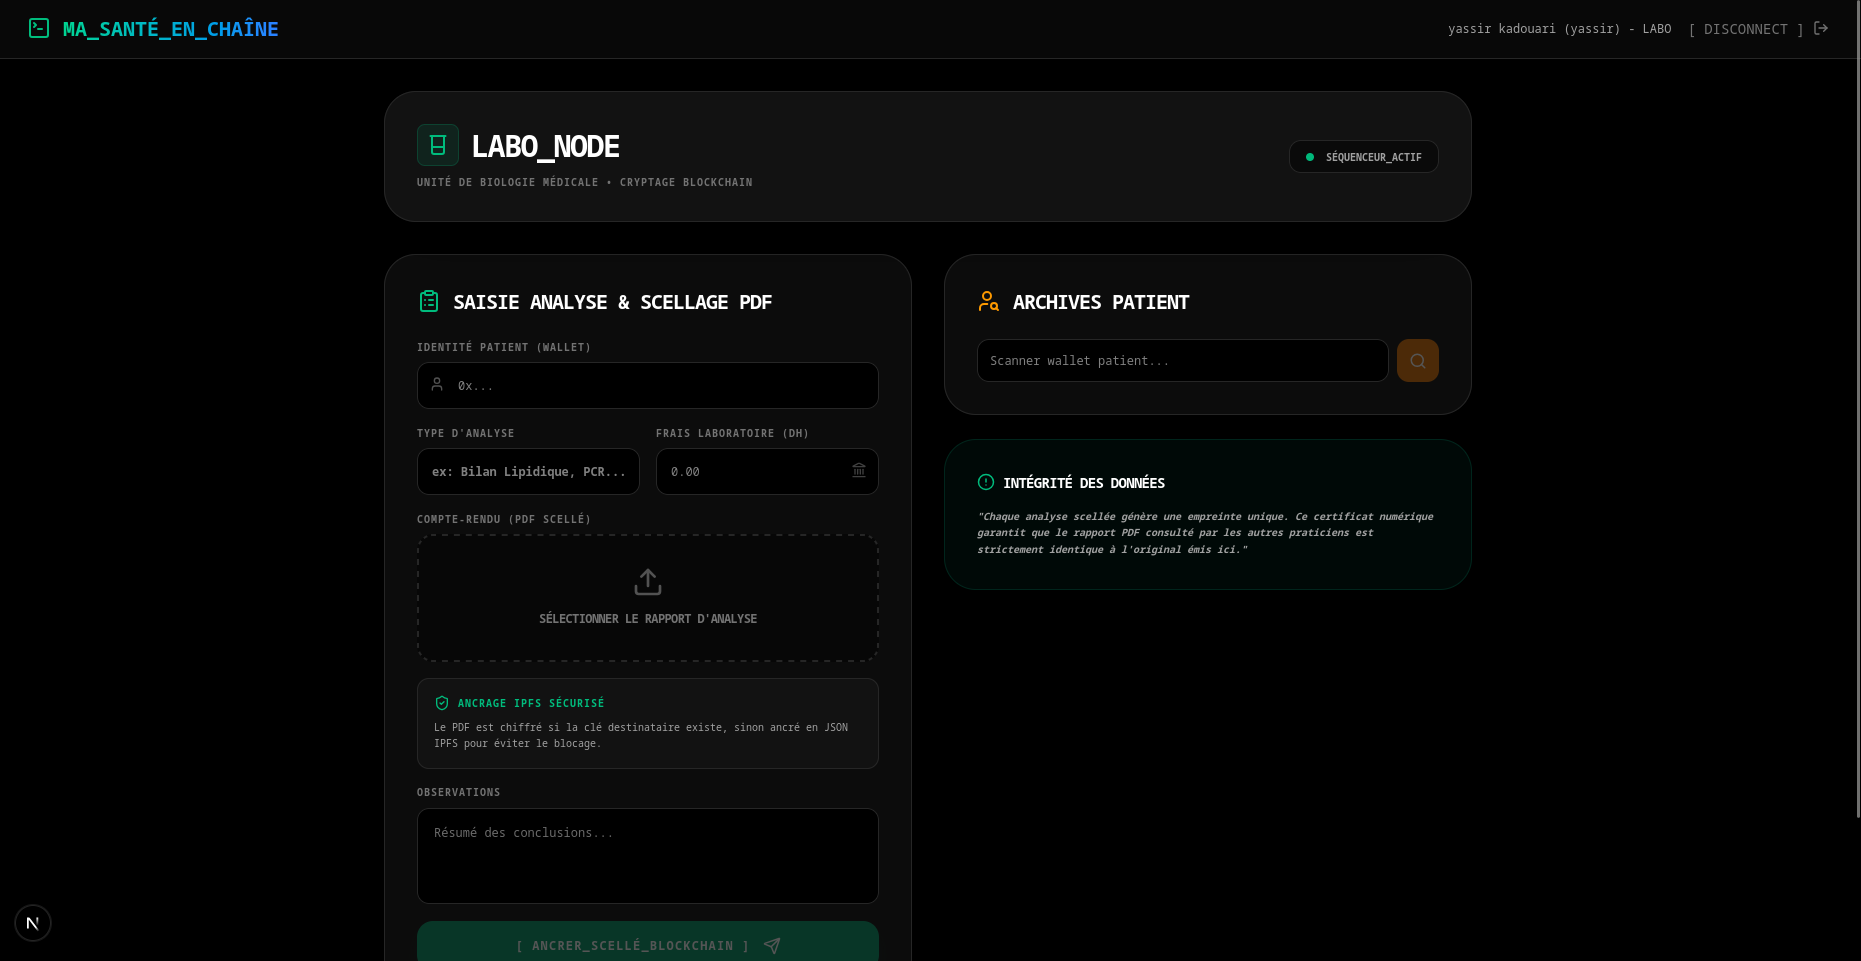
\includegraphics[width=\textwidth]{screenshots/laboratoir/dashboard.png}
    \caption{Tableau de bord Laboratoire : Soumission de résultats d'analyses}
    \label{fig:dash_labo}
\end{figure}

\subsection{Dashboard Hôpital}
L'hôpital peut créer des événements médicaux de type \texttt{OPERATION} et \texttt{VISIT}, incluant des documents PDF encodés en base64 dans le JSON chiffré.

\begin{figure}[H]
    \centering
    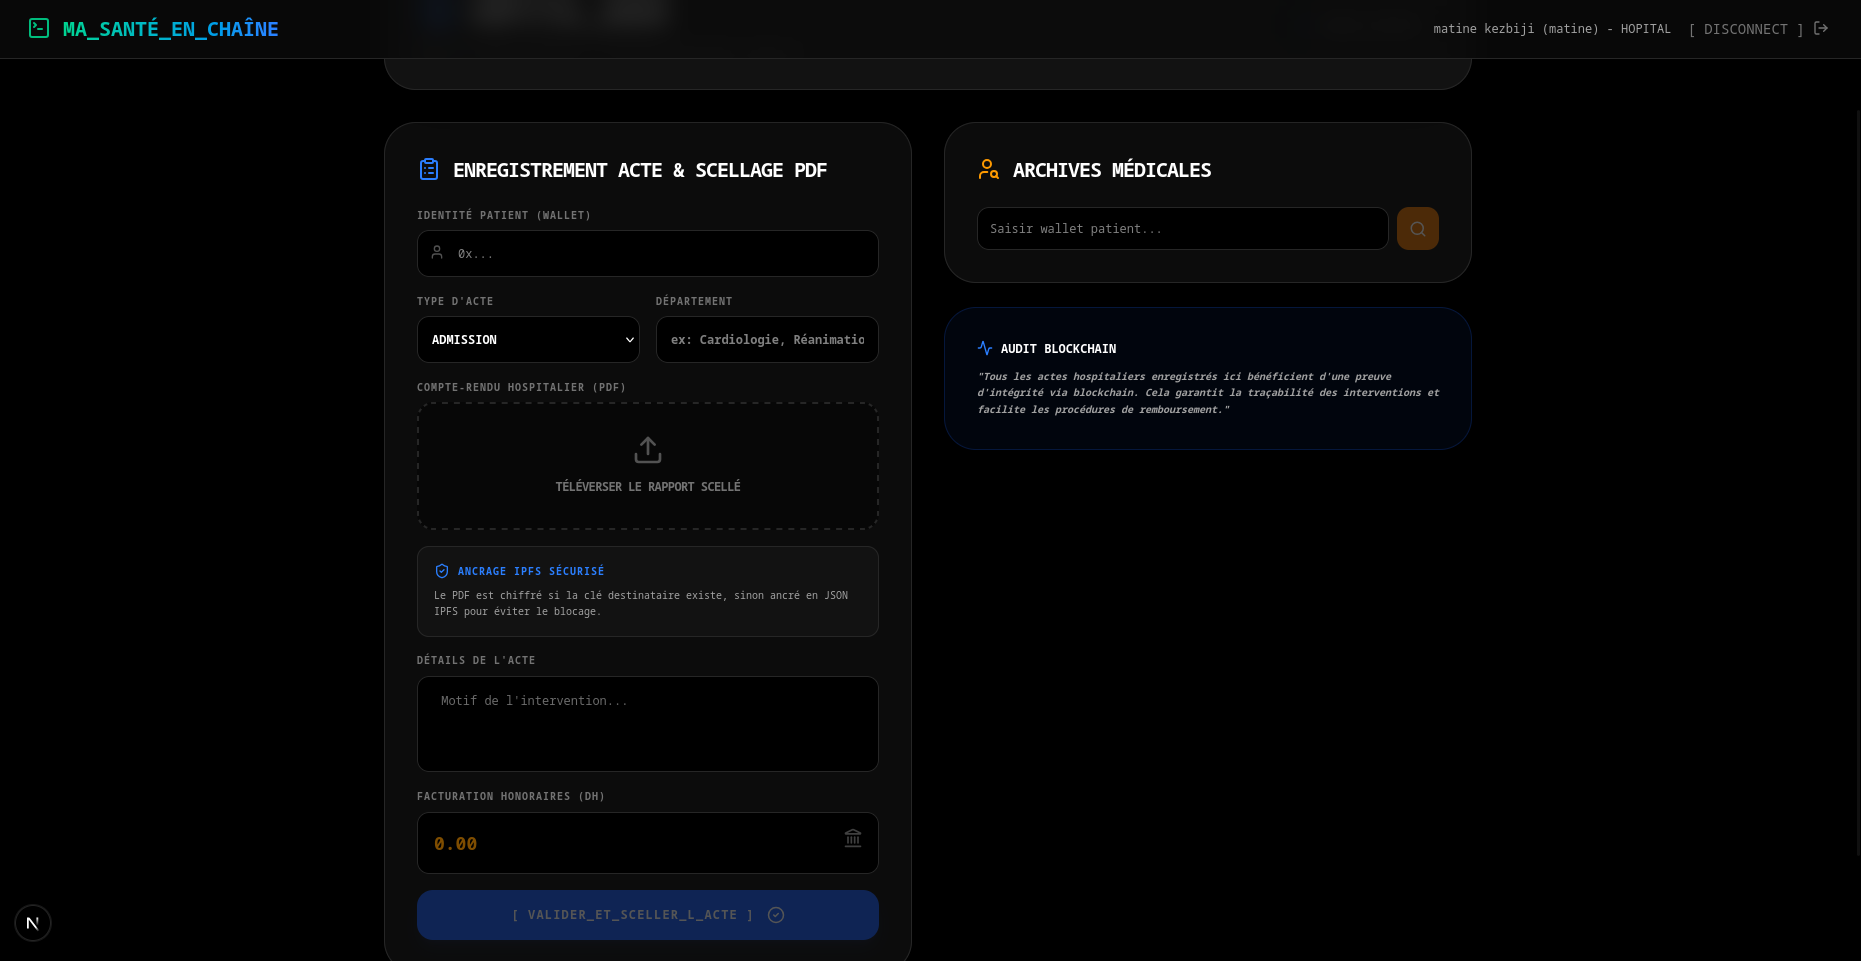
\includegraphics[width=\textwidth]{screenshots/hopital/dahsboard.png}
    \caption{Tableau de bord Hôpital : Gestion des actes médicaux}
    \label{fig:dash_hopital}
\end{figure}

\subsection{Dashboard Administrateur}
L'administrateur est l'entité de gouvernance. Il attribue les rôles on-chain aux professionnels de santé en créant des ancrages de gouvernance sur IPFS, liés aux familles de RecordId \texttt{mongo:walletroles:*}.

\begin{figure}[H]
    \centering
    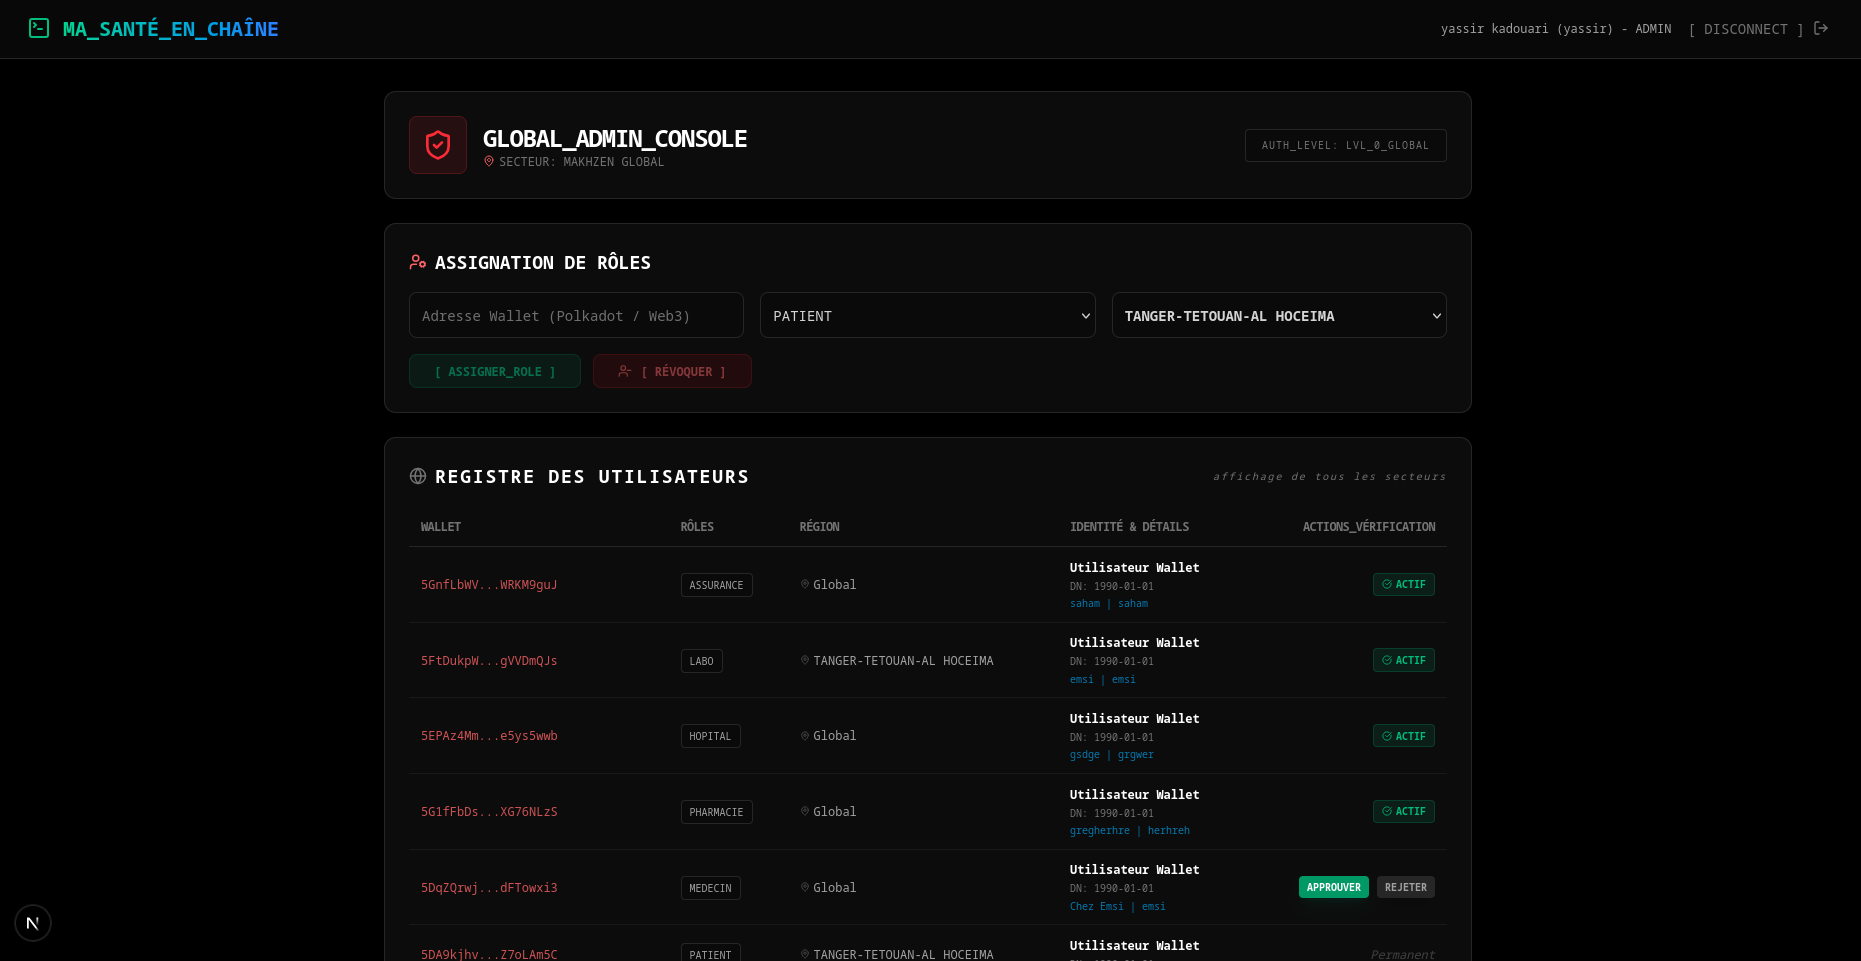
\includegraphics[width=\textwidth]{screenshots/admin/dashboard.png}
    \caption{Tableau de bord Administrateur : Gouvernance et attribution des rôles}
    \label{fig:dash_admin}
\end{figure}

\section{Défis Techniques Rencontrés et Solutions}

\begin{table}[H]
    \centering
    \caption{Défis techniques et solutions implémentées}
    \label{tab:defis}
    \begin{tabular}{|p{4cm}|p{9.5cm}|}
        \hline
        \textbf{Défi} & \textbf{Solution implémentée} \\
        \hline
        Latence IPFS et Rate Limiting & Algorithme de retry exponentiel (\texttt{withUploadRetry} dans \texttt{ipfsClient.ts}) avec fallback vers un CID temporaire \texttt{pending:*} pour ne pas bloquer le flux médical. Proxy Edge API Next.js pour contourner les blocages CORS. \\
        \hline
        Distribution des clés publiques & Le Smart Contract intègre un registre de clés publiques (\texttt{encryption\_keys} Mapping) interrogeable via \texttt{encryption\_key\_of}. Un mode dégradé (\texttt{PLAIN\_IPFS\_FALLBACK}) est activé si la clé est manquante. \\
        \hline
        Coûts de Gas imprévisibles & Le Frontend exécute des Dry Runs (simulations read-only) avant chaque transaction pour estimer le poids (WeightV2) et ajoute un buffer de 20\% (\texttt{txGasLimitFromEstimate}). \\
        \hline
        \texttt{crypto.subtle} undefined & L'API Web Crypto n'est disponible que dans un Secure Context (HTTPS ou localhost). Solution : documentation de déploiement et utilisation de tunnels ngrok pour les tests réseau. \\
        \hline
        Persistance blockchain & Migration de \texttt{--tmp} (éphémère) vers \texttt{-d ./blockchain-data} (persistant) pour conserver l'état entre les redémarrages du nœud. \\
        \hline
    \end{tabular}
\end{table}

\section{Conclusion}
Le système déployé démontre qu'il est possible de construire une application de santé résiliente, entièrement sans serveur backend propriétaire, en déléguant la vérité absolue à la blockchain et le stockage sécurisé au réseau pair-à-pair IPFS. Chaque composant — du chiffrement hybride à la vérification d'intégrité SHA-256 — contribue à un écosystème où la falsification documentaire est mathématiquement impossible.

% =======================================================
% CONCLUSION GENERALE
% =======================================================
\chapter*{Conclusion Générale et Perspectives}
\addcontentsline{toc}{chapter}{Conclusion Générale et Perspectives}

Le projet « Ma Santé En Chaîne » a constitué un défi d'ingénierie logicielle majeur mobilisant quatre membres de l'équipe pendant plusieurs mois. L'application réussie des principes du Web3 au secteur critique de la santé démontre la viabilité de ces technologies au-delà du seul domaine de la cryptomonnaie.

Au cours de ce travail, nous avons conçu et implémenté un écosystème complet comprenant :
\begin{itemize}
    \item Un Smart Contract ink! robuste en Rust gérant plus de 15 fonctions publiques (ancrages, claims, ACL, clés de chiffrement).
    \item Une bibliothèque cryptographique frontend (\texttt{medicalCrypto.ts}) implémentant un schéma d'enveloppe hybride AES-GCM + Curve25519.
    \item Un module de communication blockchain (\texttt{chainContract.ts}) avec cache, retry, estimation de Gas dynamique et gestion d'erreurs exhaustive.
    \item Sept tableaux de bord spécialisés offrant une expérience utilisateur complète pour chaque acteur du système de santé.
    \item Une architecture « Wallet-First » éliminant totalement le besoin d'un backend centralisé (Node.js/MongoDB).
\end{itemize}

L'un des acquis majeurs est la preuve qu'un pharmacien ne peut \textbf{techniquement} pas valider une ordonnance falsifiée : les mathématiques du hachage SHA-256 combinées à l'immuabilité de la blockchain Substrate l'en empêcheront toujours.

\textbf{Perspectives d'évolution :}
\begin{itemize}
    \item \textbf{Déploiement Mainnet :} Migration vers un réseau Testnet public Polkadot, puis intégration comme Parachain dédiée à la santé.
    \item \textbf{Preuves à Divulgation Nulle (ZKP) :} Intégration de zk-SNARKs permettant à un patient de prouver son éligibilité à un remboursement sans révéler la nature de son acte médical.
    \item \textbf{Intégration IoT Médical :} Permettre aux dispositifs médicaux connectés de posséder leur propre Wallet et d'ancrer directement leurs mesures sur la blockchain.
    \item \textbf{Interopérabilité HL7/FHIR :} Adapter les schémas de données pour être compatibles avec les standards internationaux d'interopérabilité en santé.
\end{itemize}

En conclusion, ce projet valide notre conviction : l'avenir des données de santé passera par des architectures décentralisées, redonnant aux patients la souveraineté totale sur leurs informations les plus sensibles.

% =======================================================
% REFERENCES
% =======================================================
\chapter*{Références}
\addcontentsline{toc}{chapter}{Références}

\begin{enumerate}
    \item Parity Technologies. \textit{Substrate Developer Documentation}. \url{https://docs.substrate.io/}
    \item Parity Technologies. \textit{ink! Smart Contracts Documentation}. \url{https://use.ink/}
    \item Protocol Labs. \textit{IPFS Documentation}. \url{https://docs.ipfs.tech/}
    \item Pinata. \textit{Pinata API Documentation}. \url{https://docs.pinata.cloud/}
    \item Polkadot.js. \textit{Polkadot API Documentation}. \url{https://polkadot.js.org/docs/}
    \item D.J. Bernstein. \textit{Curve25519: New Diffie-Hellman Speed Records}. PKC 2006.
    \item NIST. \textit{Advanced Encryption Standard (AES)}. FIPS PUB 197, 2001.
    \item NIST. \textit{Recommendation for Block Cipher Modes of Operation: GCM}. SP 800-38D, 2007.
    \item Next.js. \textit{Next.js Documentation}. \url{https://nextjs.org/docs}
    \item TweetNaCl.js. \textit{TweetNaCl.js - A port of TweetNaCl to JavaScript}. \url{https://tweetnacl.js.org/}
\end{enumerate}

\end{document}
